%\documentclass[11pt,a4paper]{article}
\documentclass[11pt
  , a4paper
  , article
  , oneside
%  , twoside
%  , draft
]{memoir}

\usepackage{control}
\usepackage[numbers]{natbib}

\newcommand{\newappendix}{%
  \refstepcounter{chapter}\chapter*{Appendix \thechapter}%
  \addcontentsline{toc}{chapter}{Appendix \thechapter}%
}

\begin{document}

\newcommand{\technumber}{
  RAON Control-Document Series\\
  Revision : v1.0,   Release : September 24, 2014}
\title{\textbf{S7-300 PLC configuration manual}}

\author{Suk Choi\thanks{choi3over4@ibs.re.kr} \\

  Rare Isotope Science Project\\
  Institute for Basic Science, Daejeon, South Korea
}
\date{\today}

\renewcommand{\maketitlehooka}{\begin{flushright}\textsf{\technumber}\end{flushright}}
%\renewcommand{\maketitlehookb}{\centering\textsf{\subtitle}}
%\renewcommand{\maketitlehookc}{C}
%\renewcommand{\maketitlehookd}{D}

\maketitle

\begin{abstract}
중이온 가속기 라온은 Allen Bradley, SIEMENS, LS산전의 PLC를 주요한 PLC로 선정하였다. 그중에서도 SIEMENS사의 PLC는 저온 plant와 함께 들어올 예정이다. 
SIEMENS사의 PLC 소프트웨어는 기존의 STEP7 및 Simulator 등 다수의 독립적인 소프트웨어들로 그 기능들이 나뉘어 있었다.그러나 최근 몇년사이 이렇게 나뉘어 있던 기능들을 하나로 통합한 새로운 소프트웨어 툴인 TIA portal을 개발하였다. 이 문서는 TIA portal을 이용하여 PLC를 설정하고 프로그래밍하는 방법을 설명하고, EPICS와의 연동을 위하여 필요한 정보를 제공하기 위하여 작성되었다.
\end{abstract}

\chapter{S7 PLC 구성 및 특징}
S7 PLC의 기본적인 특징 및 입출력 주소, PLC 프로그래밍 언어에 대하여 간단히 설명한다. 자세한 설명은 S7 PLC manual을 참고하기바란다.

\section{S7 PLC 구성}
다음 구성은 실제 프로그램에 사용하였던 구성이며, 확장 모듈은 사용하지 않았다. 많은 수의 입출력 포인트가 필요할 경우 확장 모듈을 이용하여 입출력 포인트 수를 현저히 증가시킬 수 있다. 여기에서는 S7-300 PLC를 이용하였다.

\begin{itemize}
\item Power Supplier 	    : PS 307 5A
\item CPU 		    : S7-315 2 DP
\item Communication Module  : CP343-1 Lean
\item Digital Input Module  : DI16x24VDC
\item Digital Output Module : DO16x24VDC
\item Analog Input Module   : AI2x12 bits
\item Analog Output Module  : AO2x12 bits
\end{itemize}

\section{S7 PLC와 EPICS 연동을 위해 필요한 소프트웨어}

\begin{itemize}
\item TIA portal including STEP7 professional Ver. 12.
\item WINDOWS 7 for PLC programming
\item Debian Linux 7.1 for EPICS ioc
\item EPICS BASE 3.14.12.3 \citep{EPIS_HOME}
\item s7plc EPICS deriver \citep{S7PLC_Driver_HOME}
\end{itemize}


\section{S7-300 PLC 모듈 조립}

다음은 구성된 슬롯과 각 슬롯에 위치하는 모듈의 구성 순서이다. 1번 슬롯-3번 슬롯까지는 각위치 마다 정해진 모듈을 설치해야하고, 4번 슬롯 이후로는 원하는 모듈을 원하는 위치에 위치시킬 수 있다.

\begin{itemize}
\item 1번 슬롯 : Power Supplier
\item 2번 슬롯 : CPU Module
\item 3번 슬롯 : Extention module 
\item 4번 슬롯 : CP module
\item 5번 슬롯 : Digital Input module
\item 6번 슬롯 : Digital Output module
\item 7번 슬롯 : Analog Input module
\item 8번 슬롯 : Anlaog Output module
\end{itemize}


\begin{figure}[!htb]
  \centering
  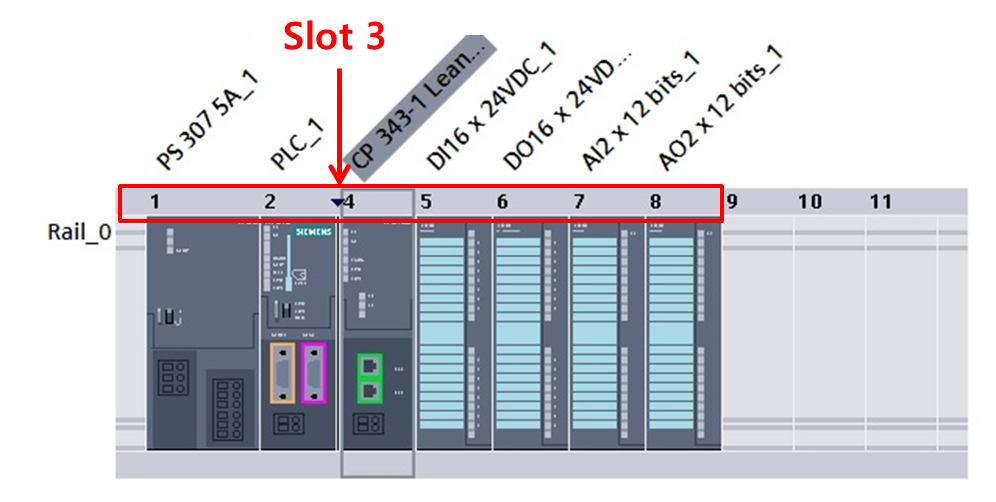
\includegraphics[width=0.96\textwidth]{./images/fig-extention-module.png}
  \caption{
            PLC module to slot configuration 
          }
  \label{fig:}
\end{figure}

S7-300 모듈은 각각의 백본을 통하여 연결되어 있고, 필요에따라 모듈의 추가 제거가 용이하도록 만들어져 있다. 모듈이 연결되는 슬롯 번호는 1번부터 시작되며, 1-3번까지의 순서는 고정되어 있지만, 4번 부터는 원하는 모듈을 원하는 위치에 삽입할 수 있다.\\
\newline Extention module(확장 모듈)은 PLC 랙의 확장시에만 필요한 모듈이다. 필요시에 3번 슬롯에 설치하고, 확장을 필요로 하지 않을 때는 생략하여 3번 슬롯을 비워둬야 한다. 3번 슬롯을 비워둔다는 의미는 물리적인 빈공간을 유지한다는 의미가 아니며, 3번 슬롯에 삽입되는 확장 모듈을 제외하고 나머지 모듈들을 연속으로 연결하라는 의미이다. 즉 3번 슬롯을 비워둔다는 의미는 소프트웨어적으로 비워둔다는 의미이다. 이렇게 확장 모듈을 제외시킨 상태에서 나머지 모듈들을 원하는 위치에 순차적으로 삽입하였을 때, PLC 모듈 설정창에서는 3번은 건너뛰고, 4번 부터 모듈이 채워지며, 특수 모듈들을 직접 컨트롤 해야 하는경우 슬롯의 번호를 확인하여 설정하면 된다.\\
\newline 다음 그림은 PLC 모듈이 설정되어 있는 상태를 나타내고 있다. 그림에서 볼수 있듯이 3번이 생략되어 있다. 3번에 위치해야할 extention 모듈이 생략되어 있기 때문에 PLC 모듈 설정화면에 3번을 제외하고 1번 2번 4번 순으로 채워져 있는 것을 확인할 수 있다.\\


\section{PLC 프로그래밍 언어}
 S7-PLC 에 지원되는 PLC 프로그래밍 언어는 다음과 같다. PLC 프로그램을 위하여 사용하는 언어는 주로 다음과 같은 3가지 언어를 사용하며, 한가지 언어만으로는 모든 기능을 사용할 수 없기때문에 사용하고자 하는 기능과 내용 그리고 표현의 수월성을 따져 3가지 언어를 적절히 섞어 사용하는 경우가 많다.

\begin{itemize}
\item Ladder Diagram
\item STL (Statement list)
\item Fuction Block Diagram
\item SCL (
\end{itemize}

\section{입출력 메모리 주소}
S7-PLC 에서의 메모리 주소의 종류는 다음과 같다.
\begin{itemize}
\item I : Input
\item Q : Output
\item M : Inner Memory 
\item C : Counter
\item T : Timer
\item L : Local memory
\item DB : Data block
\end{itemize} 
S7-PLC에서의 입출력 주소의 실제 예제는 다음과 같다.
\begin{itemize}
\item I 영역이 0-3인 경우
\begin{itemize}
\item 비트 주소 표현 I0.0 - I0.7 , I1.0 - I1.7 , I2.0 - I2.7 , I3.0 - I3.7
\item 바이트주소 표현 IB0 , IB1 , IB2 , IB3
\item 워드주소 표현 IW0 , IW2
\item 더블워드 표현 ID0 
\end{itemize}
\item Q 영역이 4-7인 경우
\begin{itemize}
\item 비트 주소 표현 Q4.0 - Q4.7 , Q5.0 - Q5.7 , Q6.0 - Q6.7 , Q7.0 - Q7.7
\item 바이트주소 표현 QB4 , QB5 , QB6 , QB7
\item 워드주소 표현 QW4 , QW6
\item 더블워드 표현 QD4 
\end{itemize}
\item M 영역
\begin{itemize}
\item 비트 주소 표현 M0.0 - M0.7 , M1.0 - M1.7 , M2.0 - M2.7 , M3.0 - M3.7
\item 바이트주소 표현 MB0 , MB1 , MB2 , MB3, ...
\item 워드주소 표현 MW0 , MW2, ...
\item 더블워드 표현 MD0, MD4, ... 
\end{itemize}
\item T 영역
\begin{itemize}
\item T0, T1, T2 , ...
\end{itemize}
\item C 영역
\begin{itemize}
\item C0, C1, C2, ...
\end{itemize}
\item DB 영역(DB11을 사용할 경우)
\begin{itemize}
\item 비트 주소 표현 : DB11.DBX0.0, DB11.DBX0.1, ... , DB11.DBX0.7, DB11.DBX1.0, ...
\item 바이트 주소 표현 : DB11.DBB0, DB11.DBB1, ...
\item 워드 주소 표현 : DB11.DBW0, DB11.DBW2, ...
\item 더블워드 주소 표현 : DB11.DBD0, DB11.DBD4, ...
\end{itemize}
\item L 영역
\begin{itemize}
\item 비트 주소 표현 L0.0 - L0.7 , L1.0 - L1.7 , L2.0 - L2.7 , L3.0 - I3.7
\item 바이트주소 표현 LB0 , LB1 , LB2 , LB3, ...
\item 워드주소 표현 LW0 , LW2, ...
\item 더블워드 표현 LD0, LD4, ...
\end{itemize}
\end{itemize}

\chapter{S7-300 PLC configuration on TIA portal}
조립된 S7-300 PLC의 순서 및 네트워트 설정 방법을 설명한다. 설정 방법은 다음의 순서를 따라가면서 직접 실행해보기를 권한다.

\section{TIA portal operate}

 Step1. PLC module을 정해진 순서에 맞게 일렬로 연결하고 백본을 연결하여 DIN RAIL에 고정한다.\\
\newline Step2. CPU 모듈의 하단에 보이는 MPI 단자에 MPI to USB 케이블을 연결하고 USB 부분을 TIA portal 프로그램이 설치된 컴퓨터에 연결한다.
\begin{itemize}
\item MPI 단자
\item DP 단자
\end{itemize}
Step3. TIA portal 프로그램을 시작하기 전에 USB에 들어있는 serial key를 key manager를 이용하여 사용하고자 하는 컴퓨터로 옮긴다. key를 옮긴 후 TIA portal 프로그램을 실행하면 key를 자동으로 인식되며, 프로그램이 정상동작된다. 만일 key가 컴퓨터 상에 존재하지 않을 경우 프로그램 실행 단계에서 메세지 박스로 key가 존재하지 않음을 통보받게되며, 프로그램은 종료된다. key는 USB 로 제공되나 USB 상에서는 프로그램을 실행하지 못하며, 프로그램을 실행할 하드웨어로 이동후 사용해야 한다.

\section{PLC hardware configuration on TIA portal software}
Step1. TIA portal 프로그램을 실행하면 다음 FIgure 2 같은 화면이 나타나는데, 이때 그림의 1번과 2번의 \verb|Project->New|를 눌러 새프로젝트를 시작한다.\\
\begin{figure}[!htb]
  \centering
  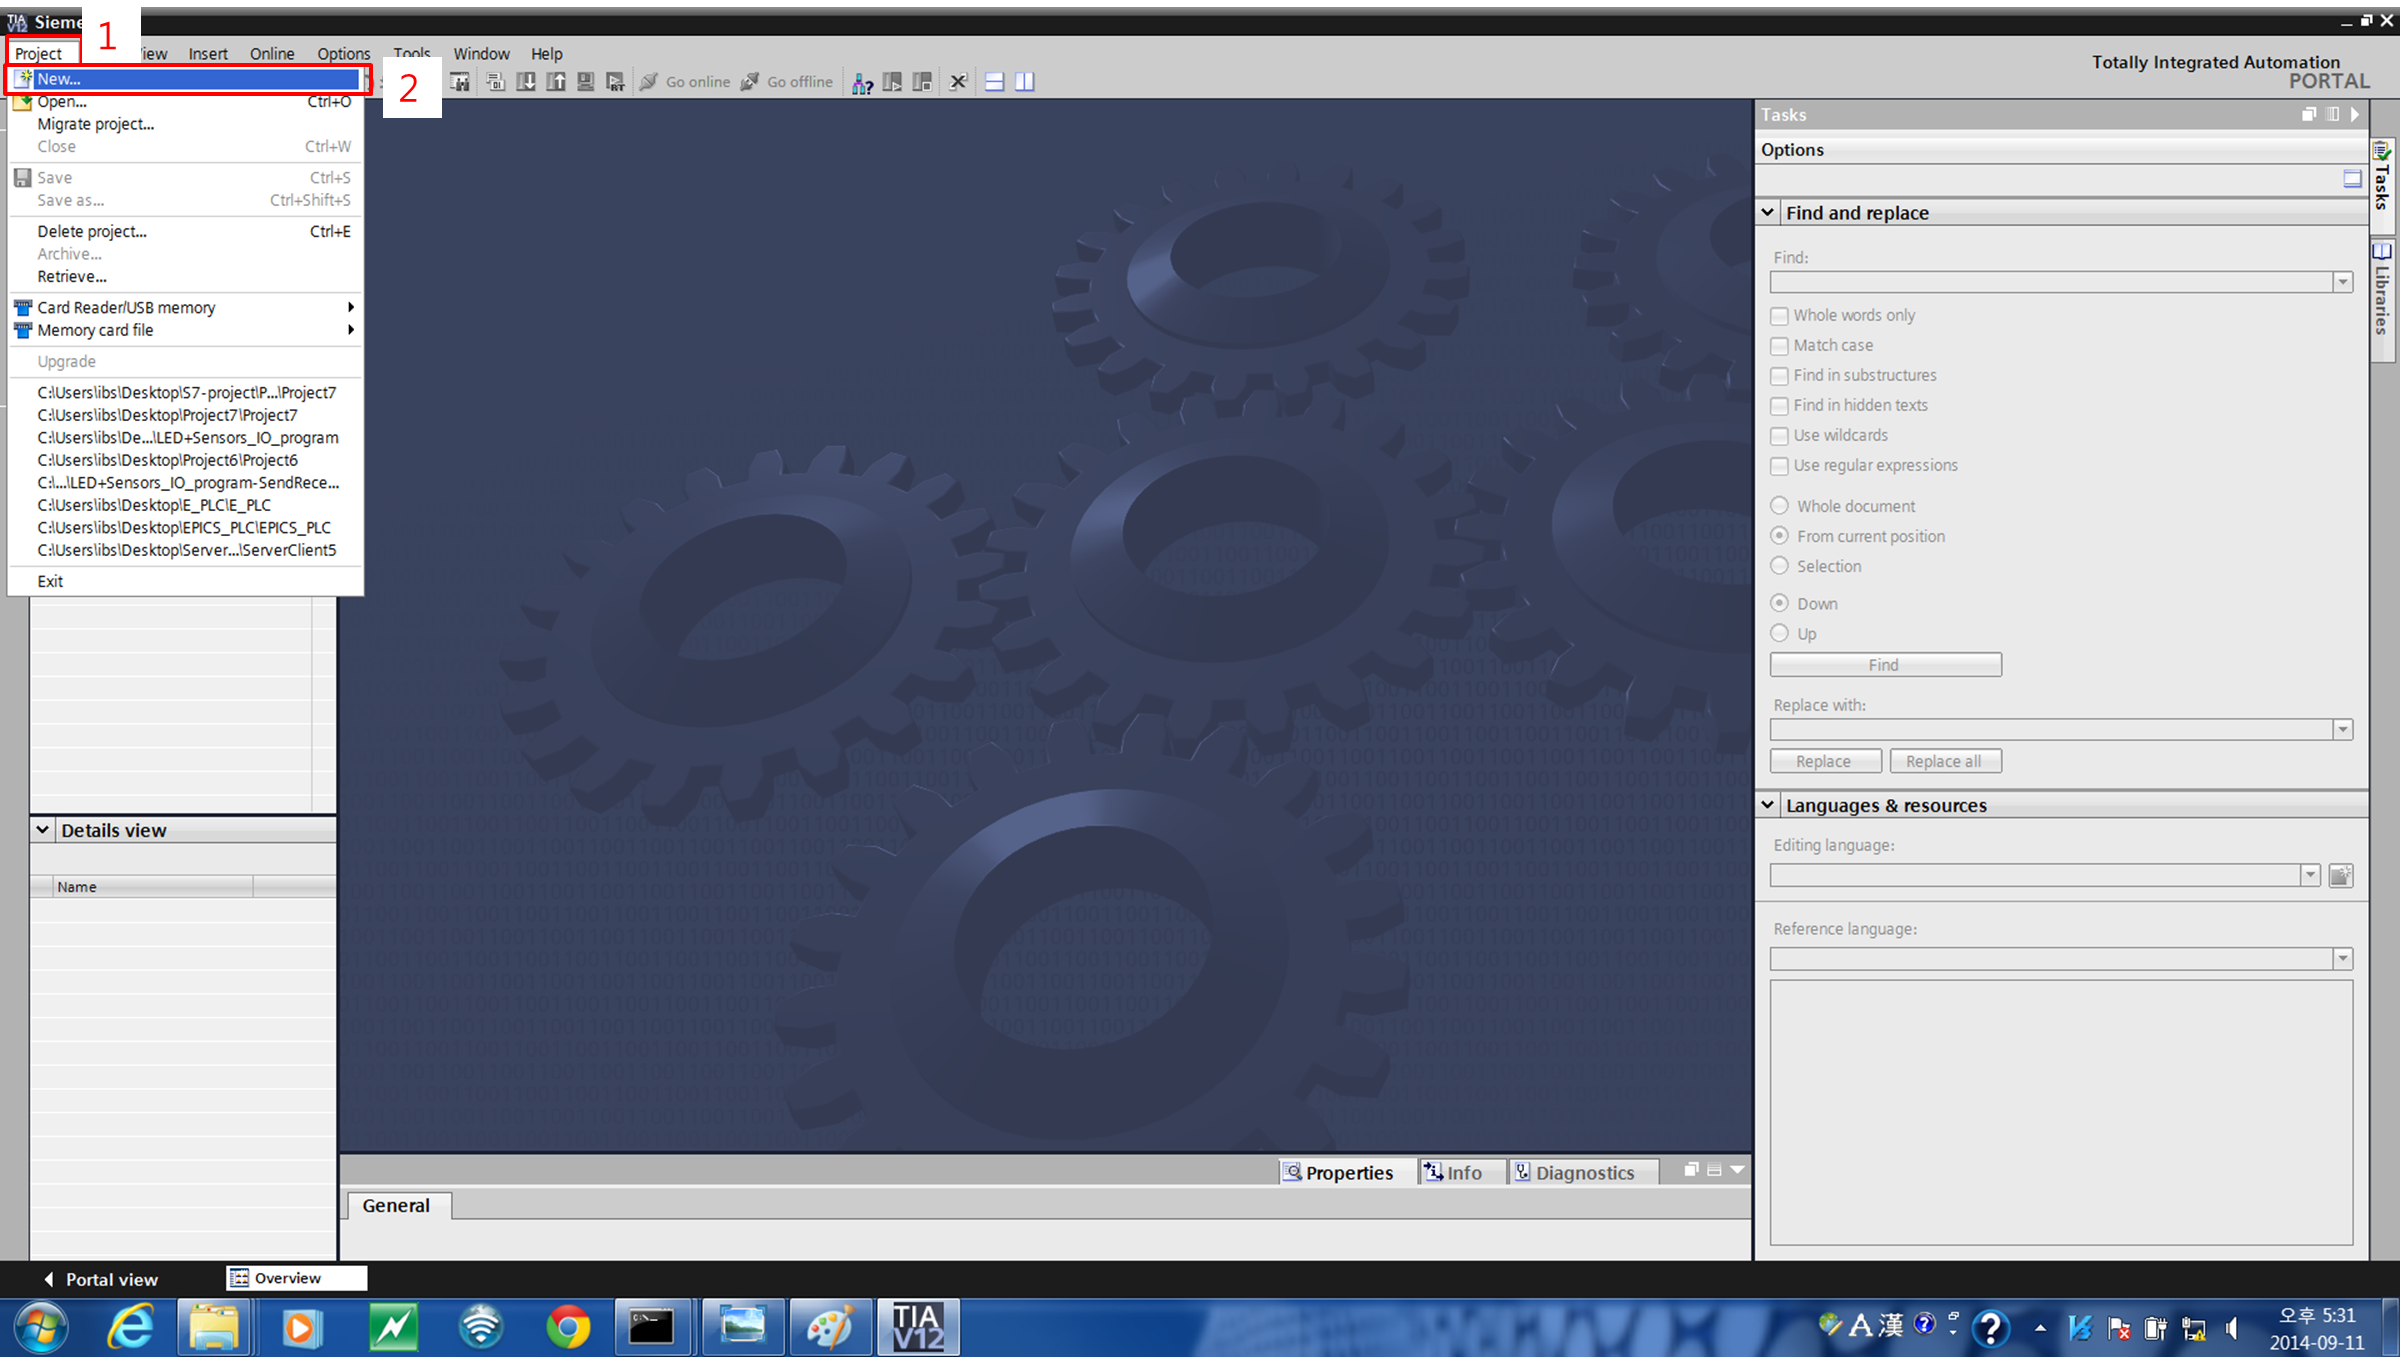
\includegraphics[width=0.96\textwidth]{./images/fig-project-click.png}
  \caption{New Project}
  \label{}
\end{figure}
\newline Step2. 새프로젝트 시작을 선택하면 Figure 3 같은 프로젝트 시작 화면이 나타난다. 이때, 3번 박스에 표시된 부분에 Project name과 Path, Author 및 Comment와 같은 정보를 기록한 후 \verb|Creat|를 누른다.\\
\begin{itemize}
\item 기록할 내용
\begin{itemize}
\item Project name 
\item Path
\item Author
\item Comment
\end{itemize}
\end{itemize}

\begin{figure}[!htb]
  \centering
  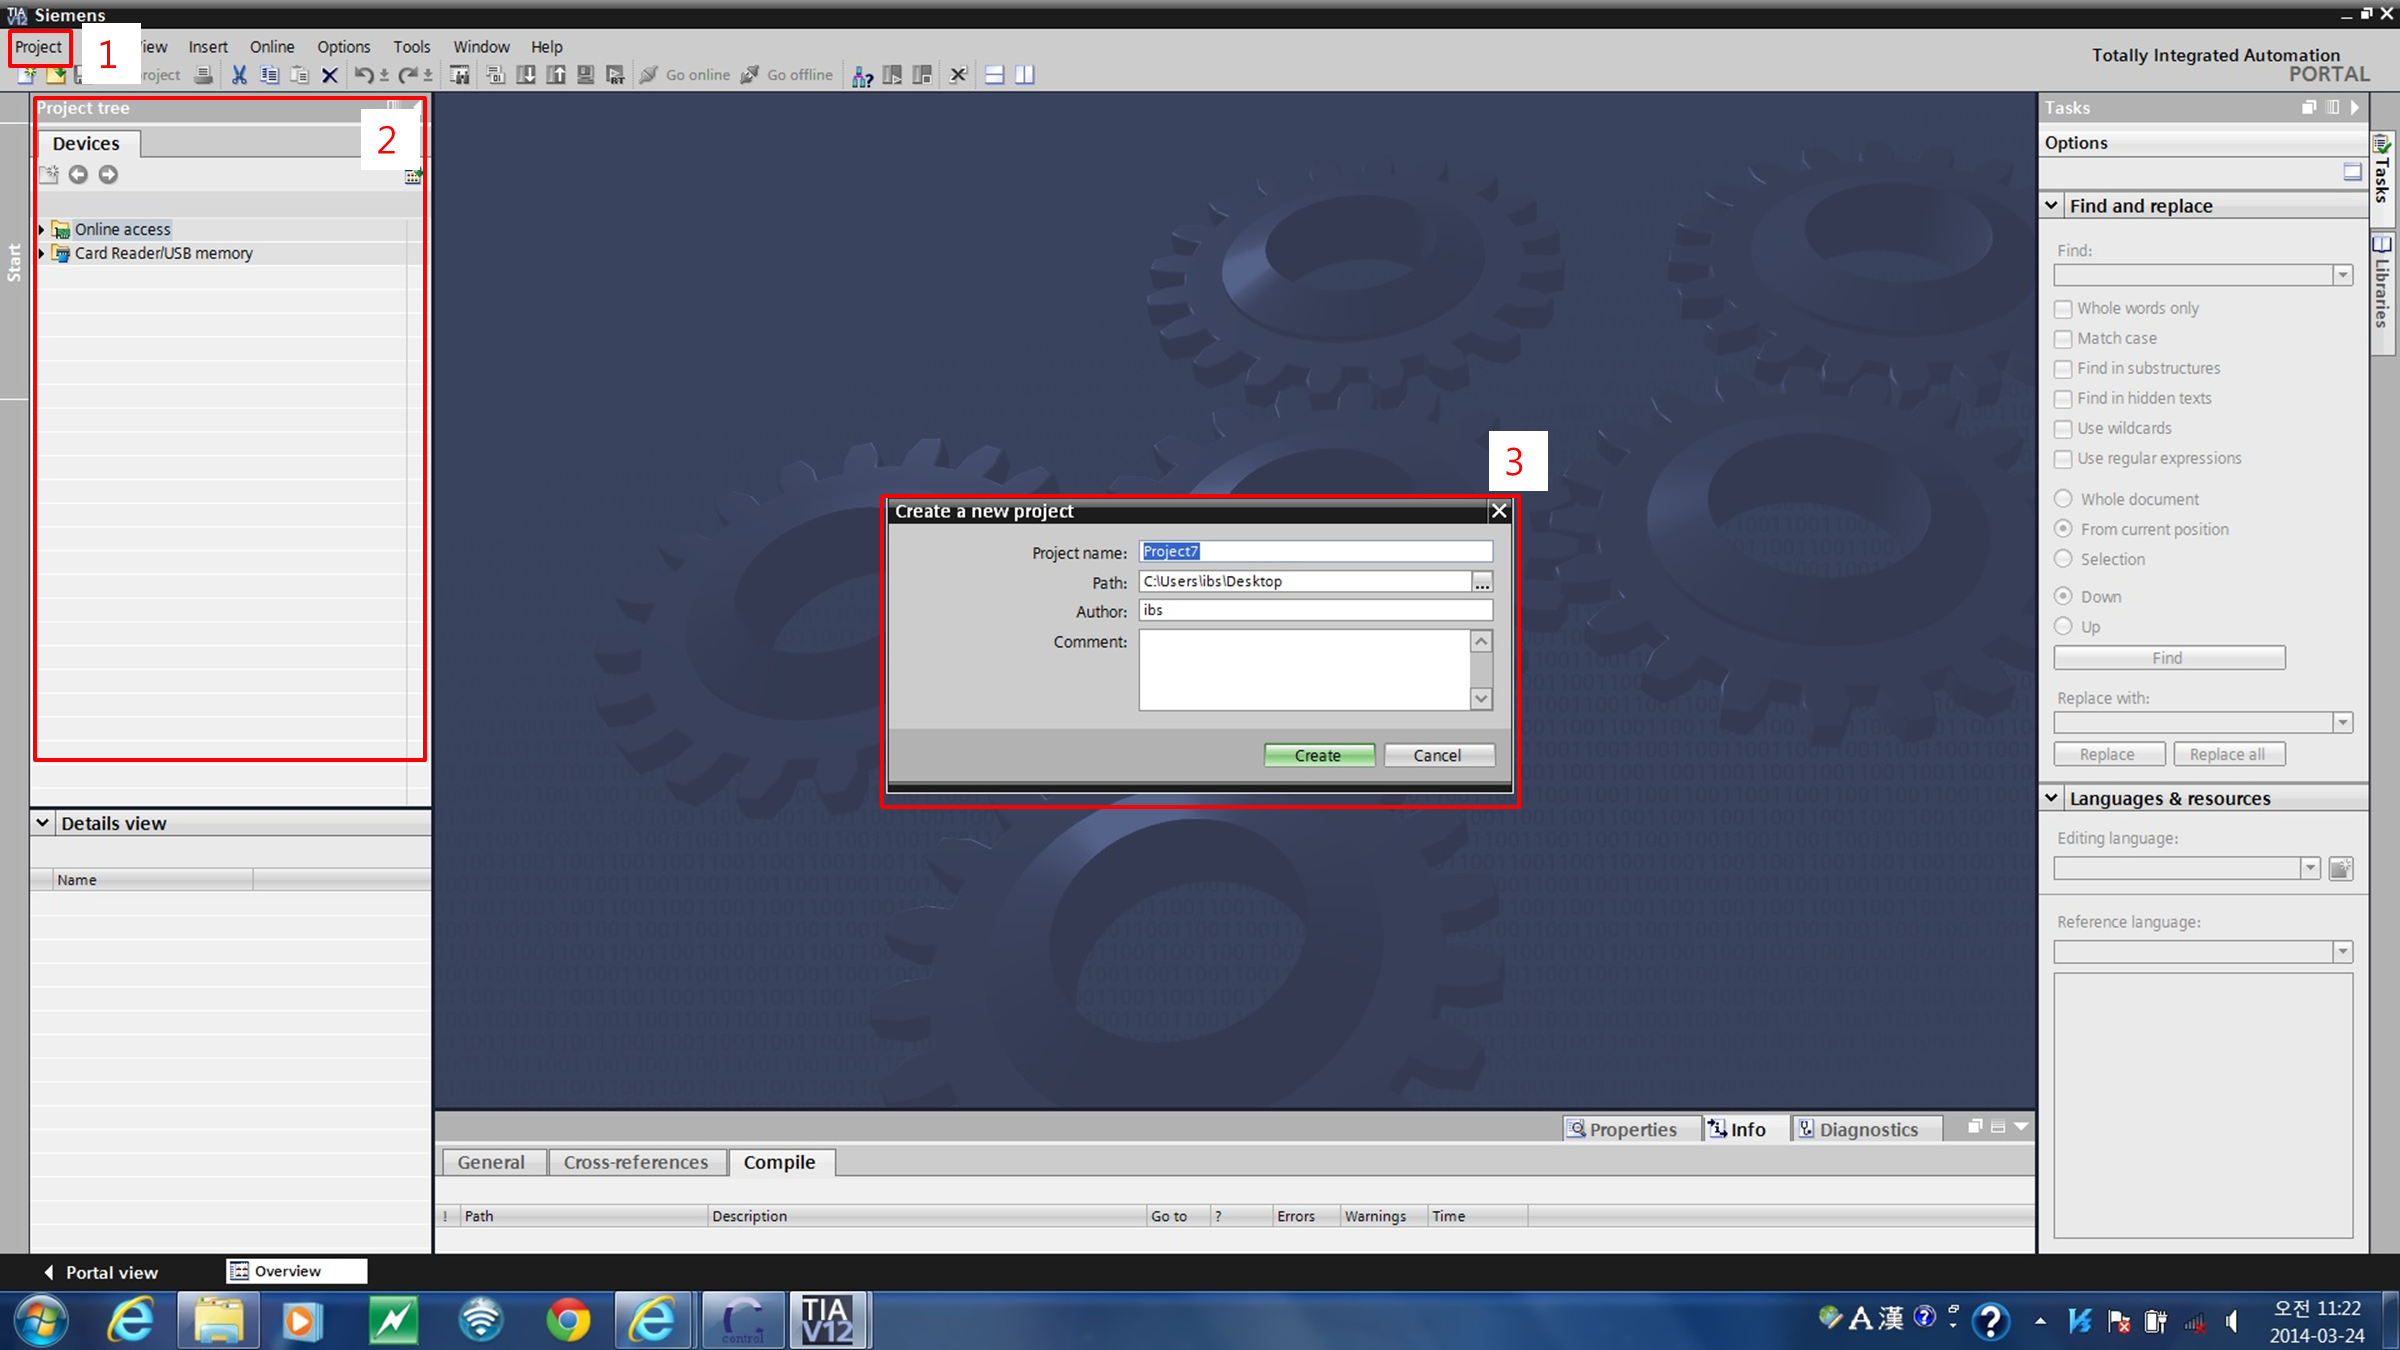
\includegraphics[width=0.96\textwidth]{./images/fig1-new-project.png}
  \caption{Creat New Project}
  \label{}
\end{figure}

Step3. 새프로젝트를 시작하면 Figure 4의 왼쪽에 \verb|Project tree|가 나타나고, \verb|Devices| 텝 안에 입력한 프로젝트 이름 밑으로 1번 박스와 같은 \verb|Add new device|항목이 나타나는데 이 것을 더블클릭한다. \verb|Add new device|를 더블클릭하면 화면 중앙의 박스와 같은 \verb|Add new device|박스가 나타나면 이 때 \verb|Device name|에 PLC set의 고유 이름을 임의대로 지정해준다. \verb|Controllers| 를 클릭하면 3번 과같이 컨트롤러의 종류들이 리스트로 나타나는데 이 항목들 중 설치하고자 하는 모듈을 선택하면 되는데, CPU 모듈을 클릭하여 리스트 중에서 설정하고자 하는 CPU의 종류를 선택하고 구입한 모듈 제품의 Order number에 해당하는 목록을 확인하여 정확하게 선택한다. 각각에 해당하는 모듈의 Order number를 클릭하면 우측 4번 박스에 선택한 모듈의 상세 정보가 나타난다. 이때 Order number 와 Version정보가 설치하고자 하는 모듈의 제품 정보와 일치하는지를 확인한다.\\
\begin{itemize}
\item 체크 항목
\begin{itemize}
\item Order number
\item Version information
\end{itemize}
\end{itemize}

Order number나 Version정보가 다를 경우 오류를 발생할 수 있다.여기까지 되었다면 \verb|OK|를 클릭하여 다음 단계로 넘어간다.\\
\begin{figure}[!htb]
  \centering
  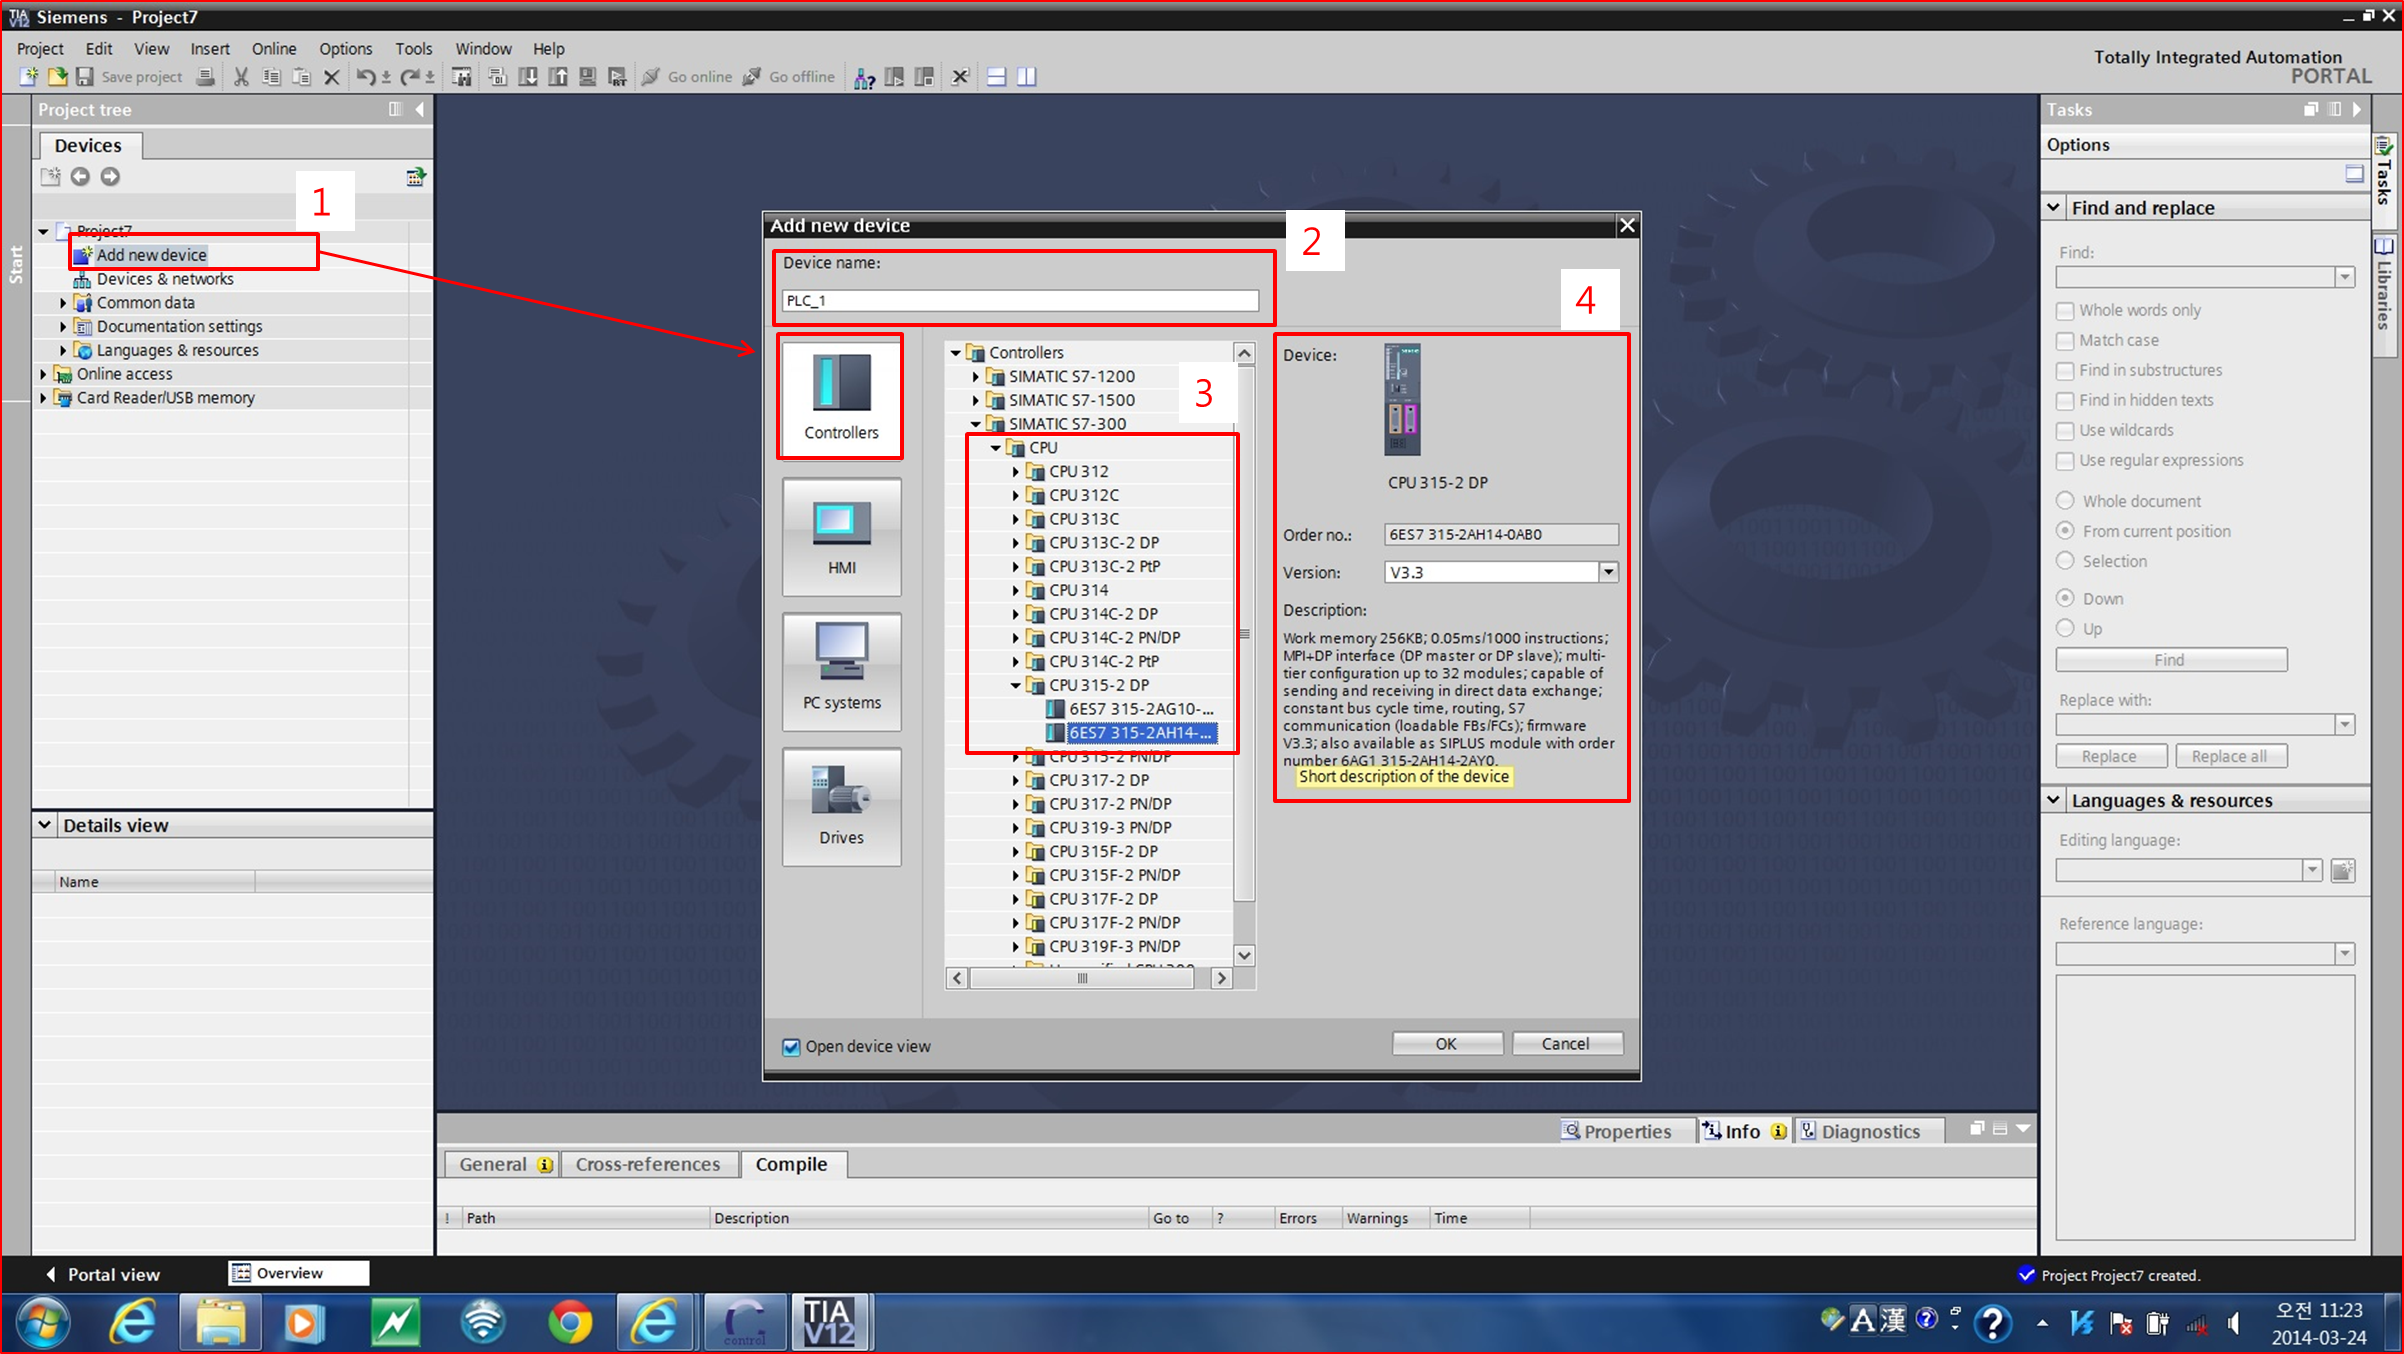
\includegraphics[width=0.96\textwidth]{./images/fig2-cpu-select.png}
  \caption{CPU configuration}
  \label{}
\end{figure}
\newline Step4. 정상적으로 CPU 모듈의 정보가 입력되었다면 Figure 5 에 나오는 것과 같이 2번 슬롯에 CPU 모듈이 들어가 있는 것을 확인할 수 있다. 또한 동시에 하단의 "Device overview"창에 입력한 CPU의 상세한 정보와 현재 연결된 interface 타입과 Oeder number, Version정보와 같은 모든 정보를 확인할 수 있다.\\
\begin{itemize}
\item CPU information
\begin{itemize}
\item Interface type
\item Order number
\item Version inforamtion
\end{itemize}
\end{itemize}
\begin{figure}[!htb]
  \centering
  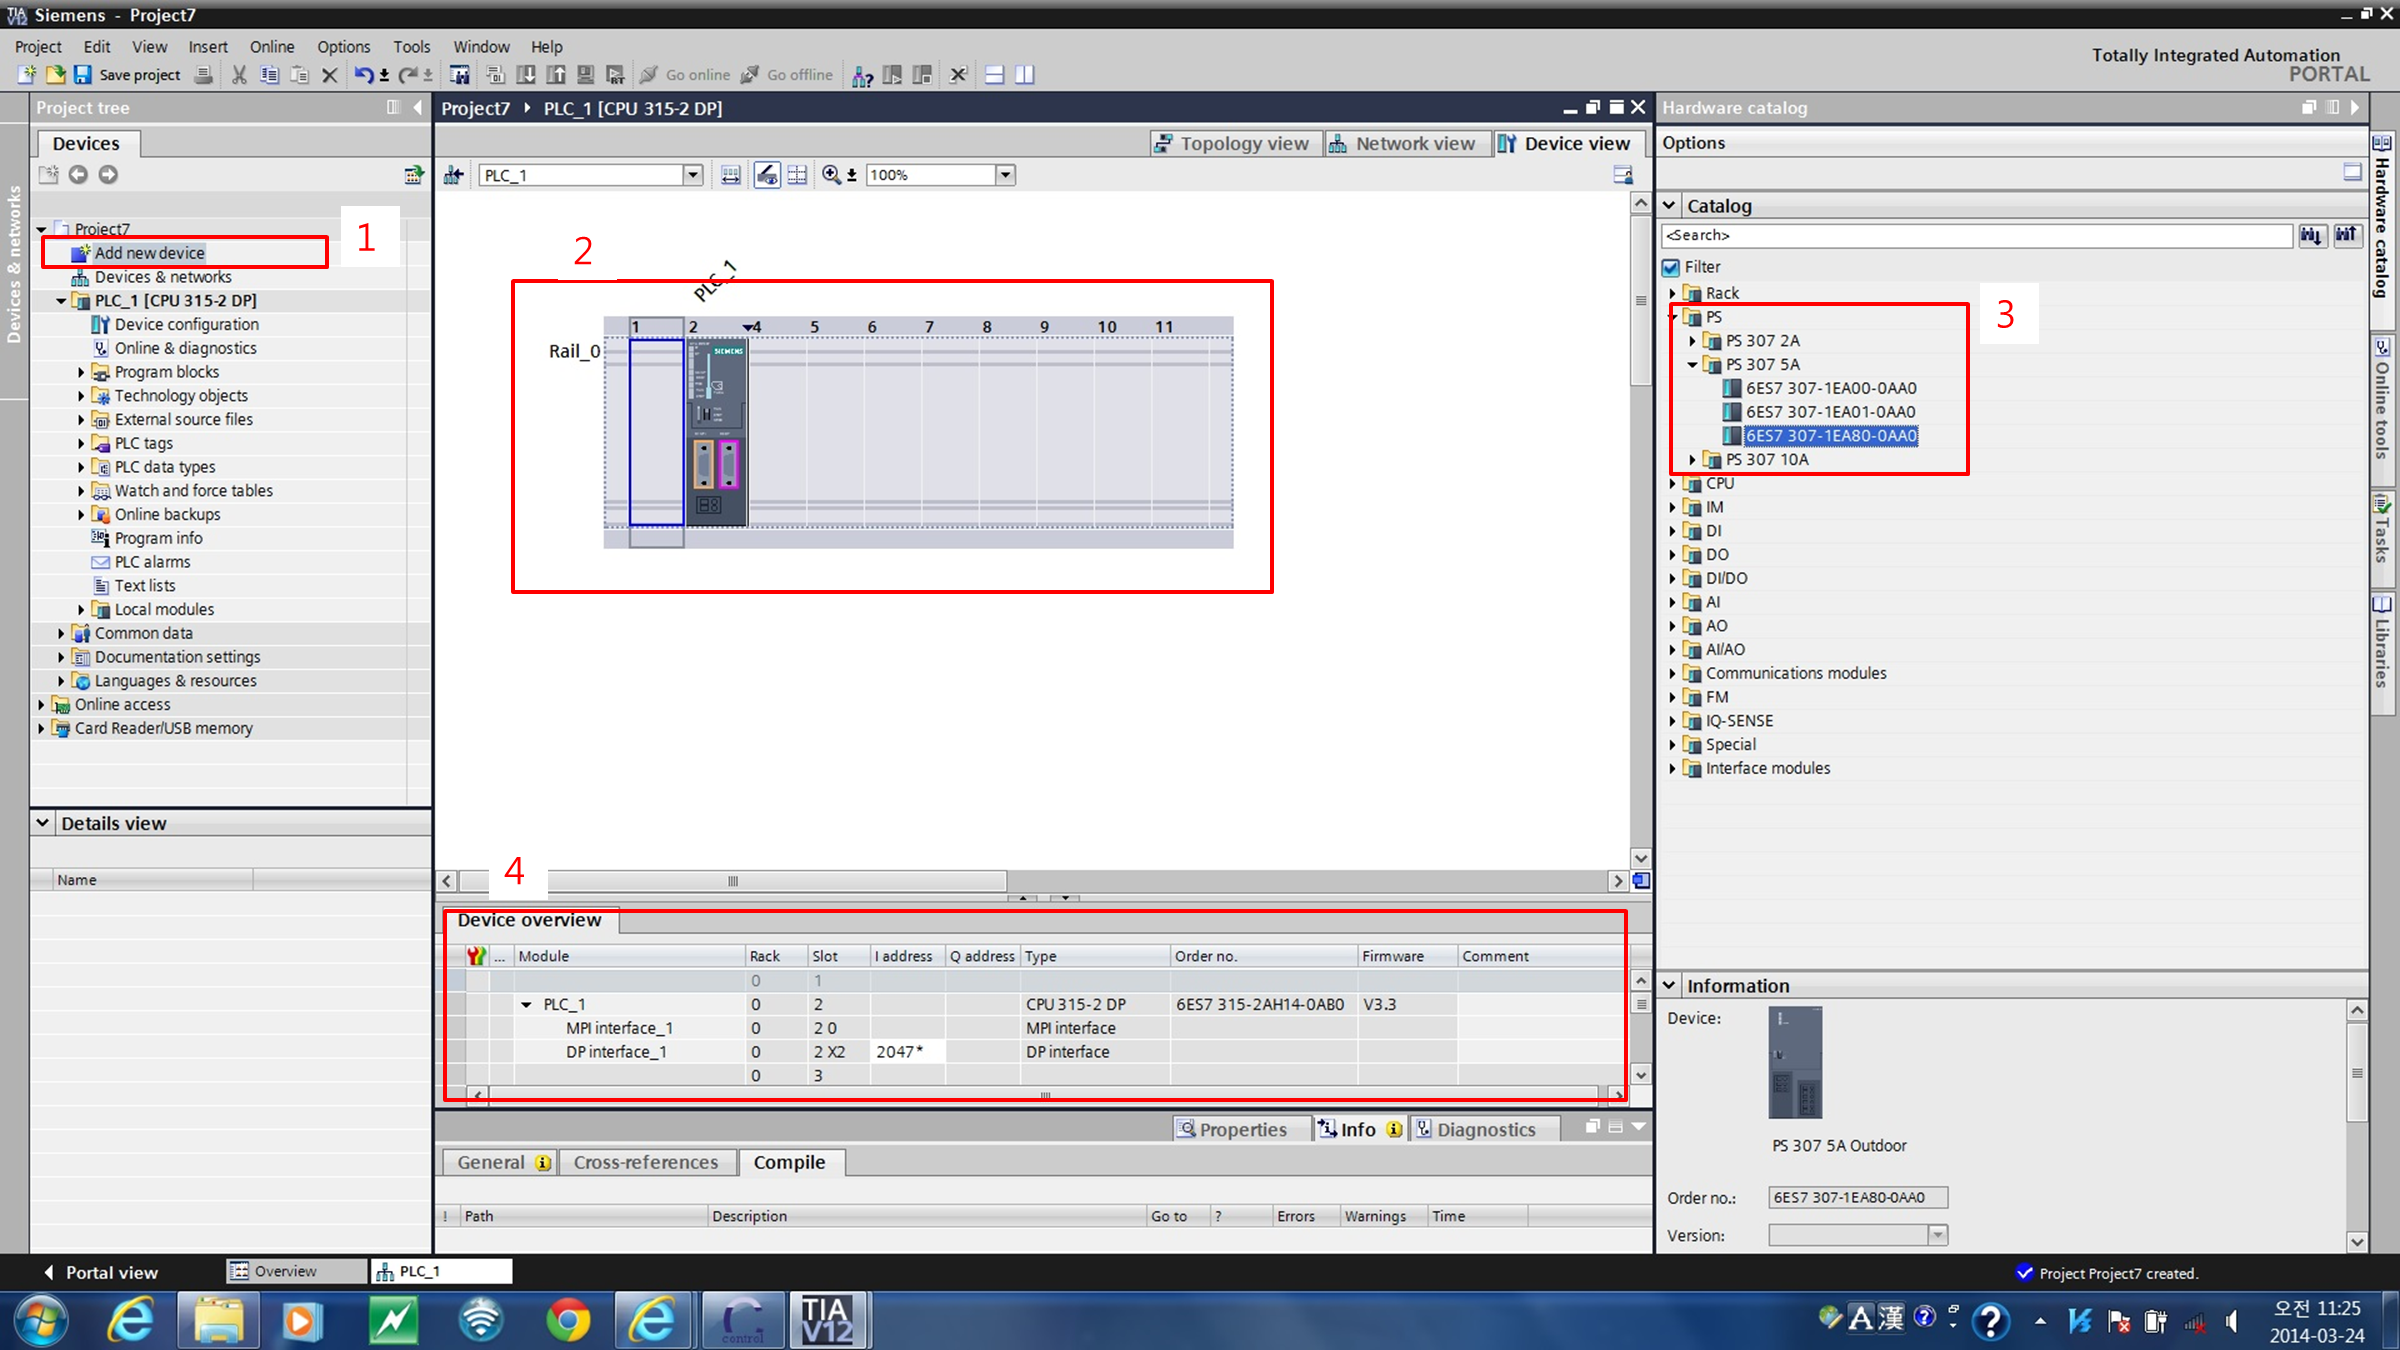
\includegraphics[width=0.96\textwidth]{./images/fig3-power-select.png}
  \caption{Power supplier configuration}
  \label{}
\end{figure}
Step5. 이제 Power supplier 모듈을 설정해보자, Power supplier 모듈은 정확하게 슬롯1번에 위치해야한다. 1번 슬롯을 클릭하여 선택한후 우측의 3번 박스를 확인하면 모듈에 관한 정보들이 리스트로 펼쳐져 있는 것을 확인할 수 있고, 그중 원하는 모듈을 선택하여 CPU 모듈을 설정할 때와같은 방법으로 정확한 Order number와 Version을 선택하여 더블클릭하면 CPU 모듈을 설정할 때와 같이 모듈의 위치가 정해진다. 3번 슬롯은 Extention모듈의 위치로 우리는 Extention을 하지 않을 것이므로 4번 슬롯으로 넘어간다. \\
\newline Step6. 4번 슬롯에는 이더넷을 통한 통신 모듈을 설정하도록하겠다. 4번 슬롯의 설정이 EPICS와의 통신 방법에 영향을 주므로 주의깊게 설정하도록 한다. 앞서 설정한 모듈들과 같은 과정으로 일단 CP 모듈을 선택하여 삽입한다. CP 모듈을 설정하고 Figure 6 에서 처럼 \verb|Device overview|에서 상세 내용을 확인한다. \\
\begin{figure}[!htb]
  \centering
  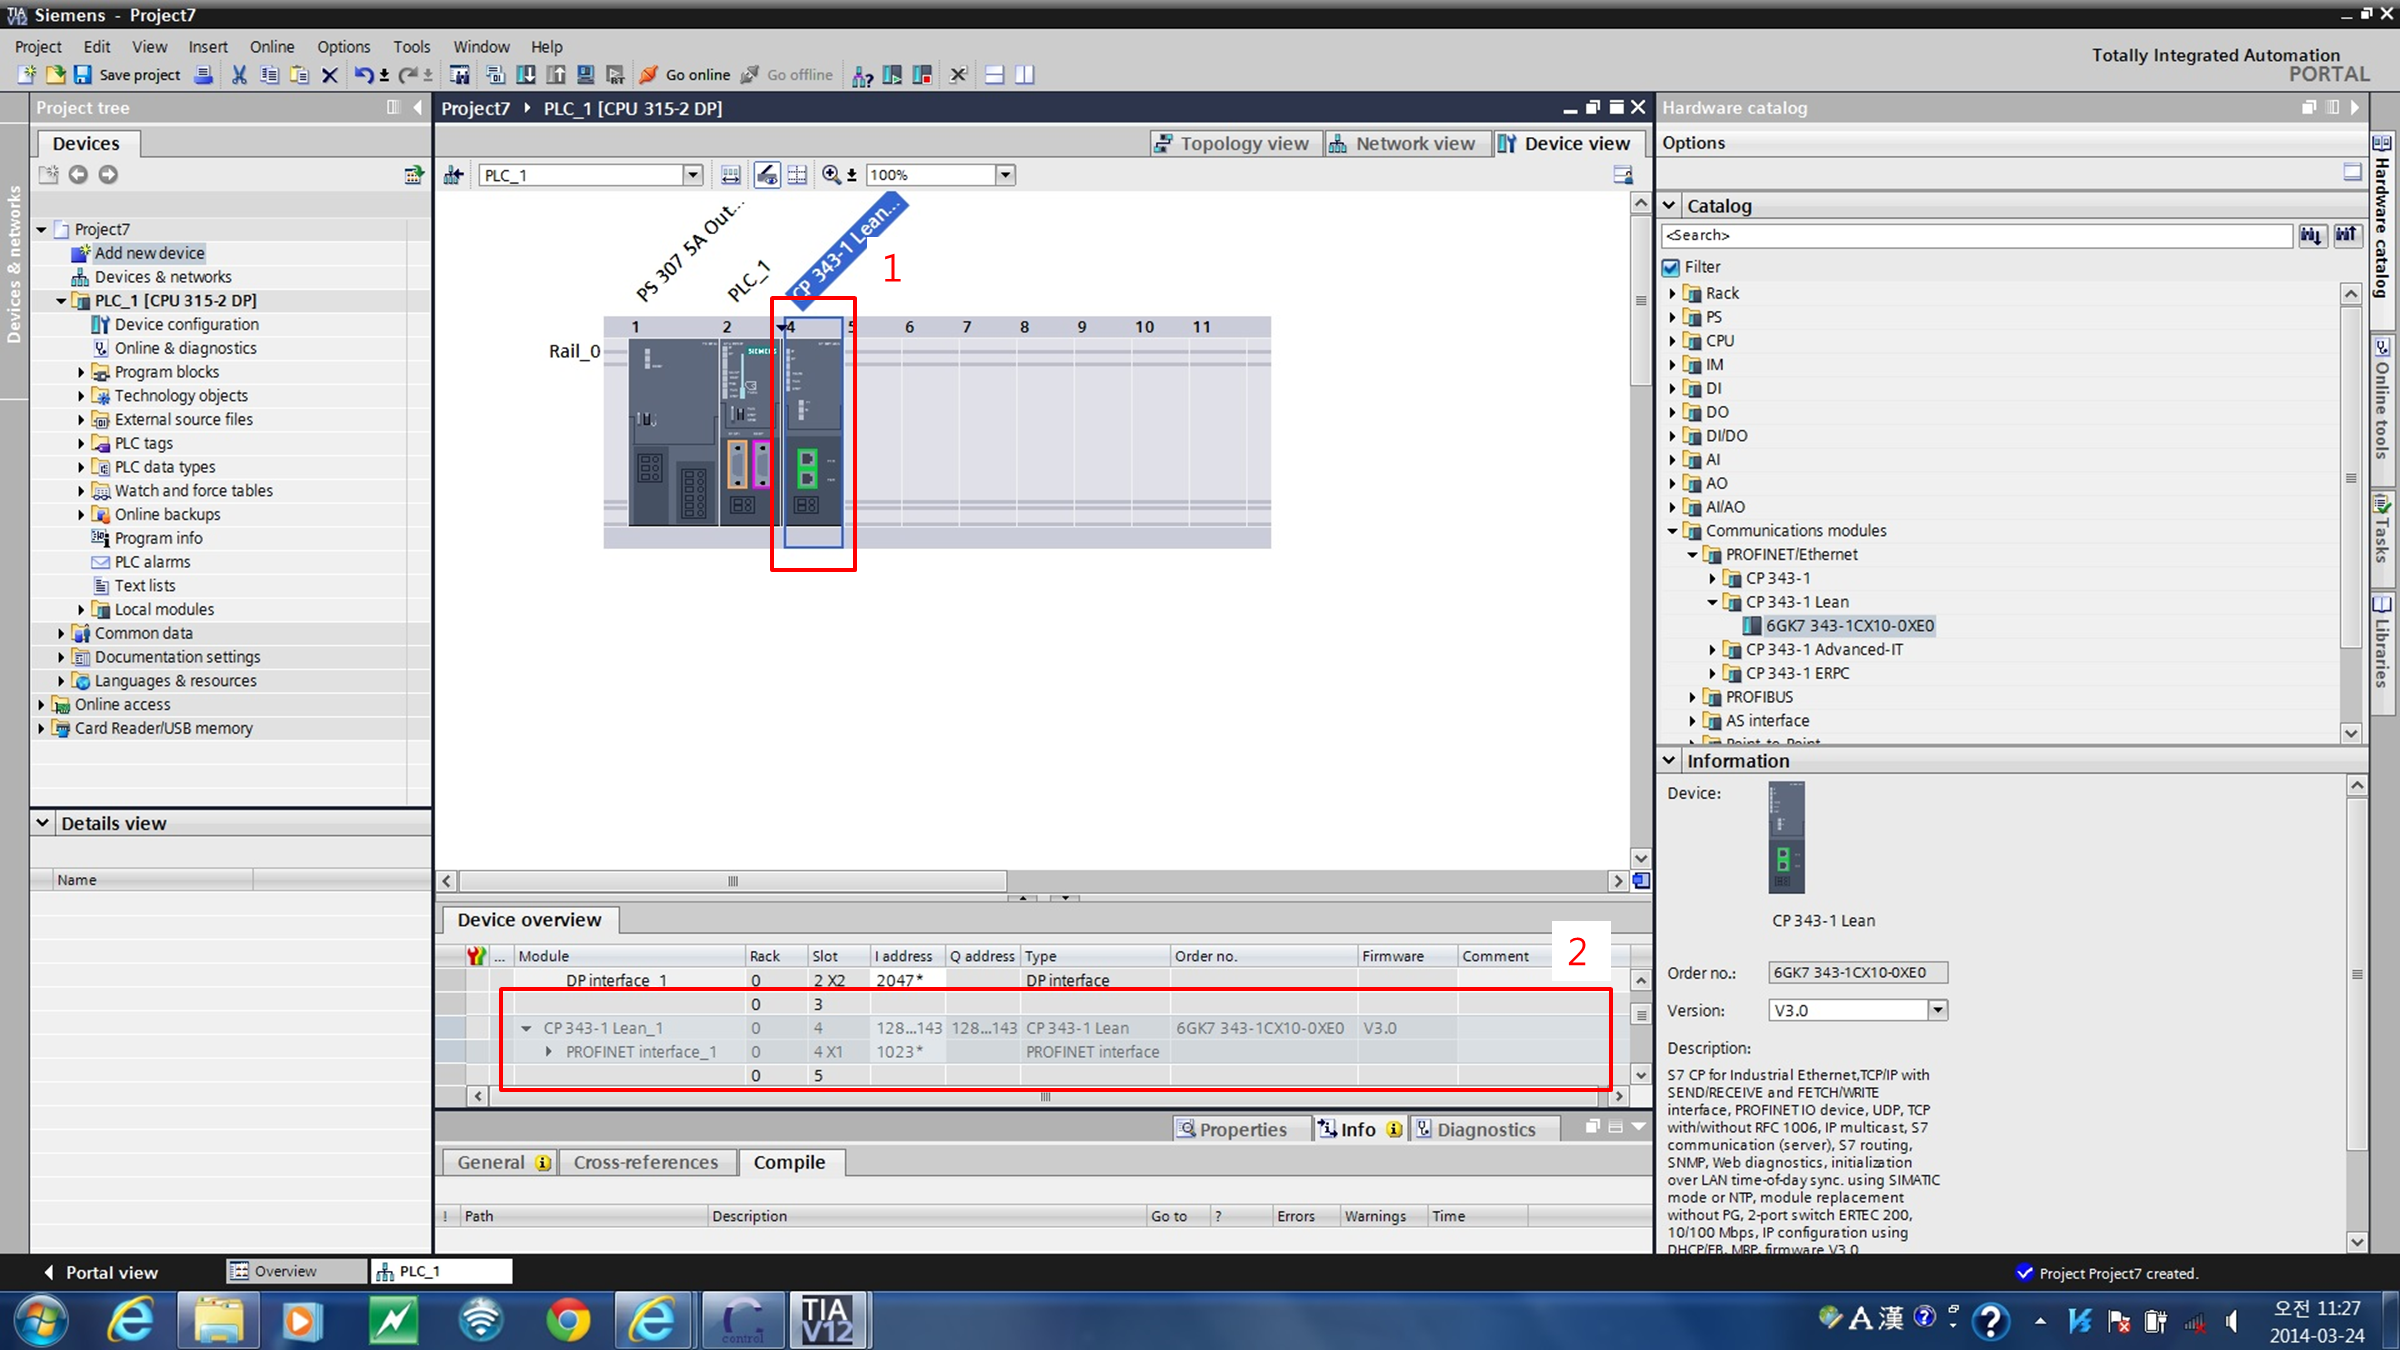
\includegraphics[width=0.96\textwidth]{./images/fig4-cp-select.png}
  \caption{Communication module configuration}
  \label{}
\end{figure}
\newline Step7. CP 모듈을 설정하였으면, 4번 슬롯을 한 번 클릭한다. Figure 7 하단의 \verb|Properties| 텝을 선택한 후 2번 박스와 같은 \verb|General| 텝을 선택한 후 다시 3번 박스와 같이 \verb|Ethernet Addresses|를 클릭하면 4번 박스의 정보가 나타나고 그중 5번 박스 부분에 있는 IP address와 Subnet masks를 설정한다. IP address는 설정 되었으므로 이더넷을 통한 통신이 가능하게 되었다.\\
\begin{figure}[!htb]
  \centering
  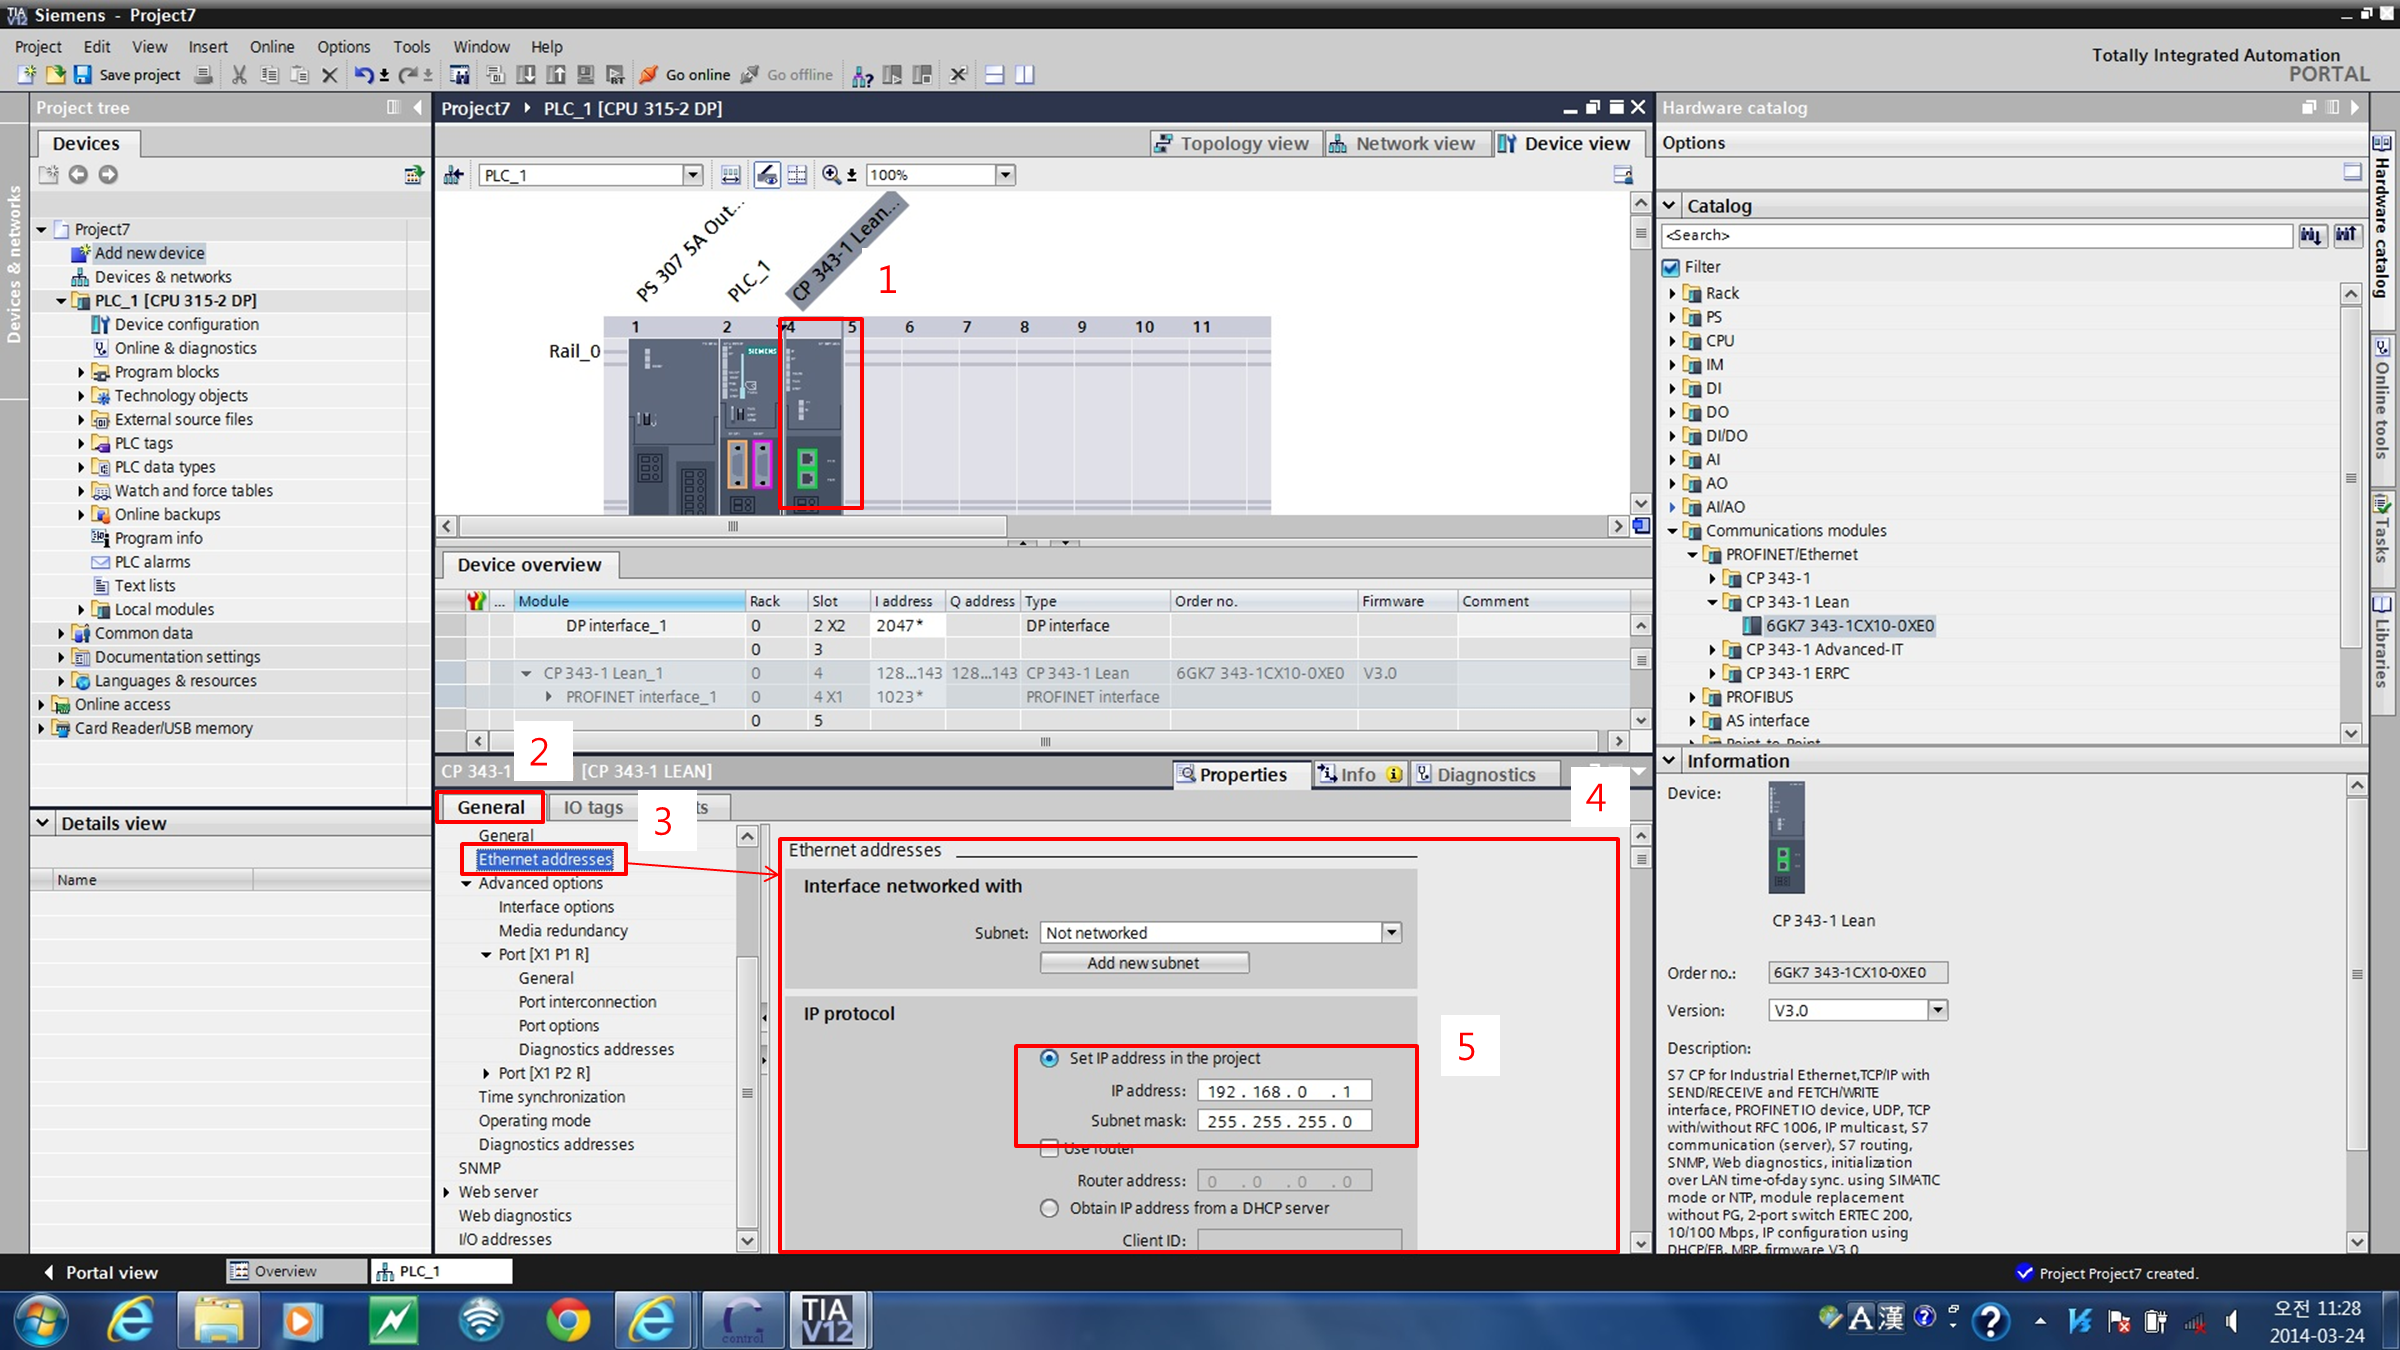
\includegraphics[width=0.96\textwidth]{./images/fig5-IPADD-set.png}
  \caption{IP address configuartion}
  \label{}
\end{figure}
\newline Step8. 이번 Step은 EPICS와 S7 PLC의 통신에 있어서 매우 중요한 부분이다. Figure 8 의 1번 박스와 같이 \verb|Devices networks|를 클릭한다. 두번 클릭하면 중앙에 그림과 같은 내용의 네트워크 설정 상태가 나타난다. 이때, 5번 박스의 \verb|Network view| 텝을 선택하면 CP 모듈의 네트워크 설정에 대한 자세한 상황을 한눈에 볼 수 있다.\\ 
\newline 2번 박스에서 Connection을 선택하고, 3번 박스의 리스트에서 \verb|TCP connection|을 선택한다. 그리고 4번 박스로 표시된 부분의 작은 연두색 상자를 마우스로 두번 클릭한다. 만약 \verb|TCP connection|이 정상적으로 설정되었다면 7번 박스와 같이 \verb|Connections|  텝에 상세 내용이 나타난다. \\
\begin{figure}[!htb]
  \centering
  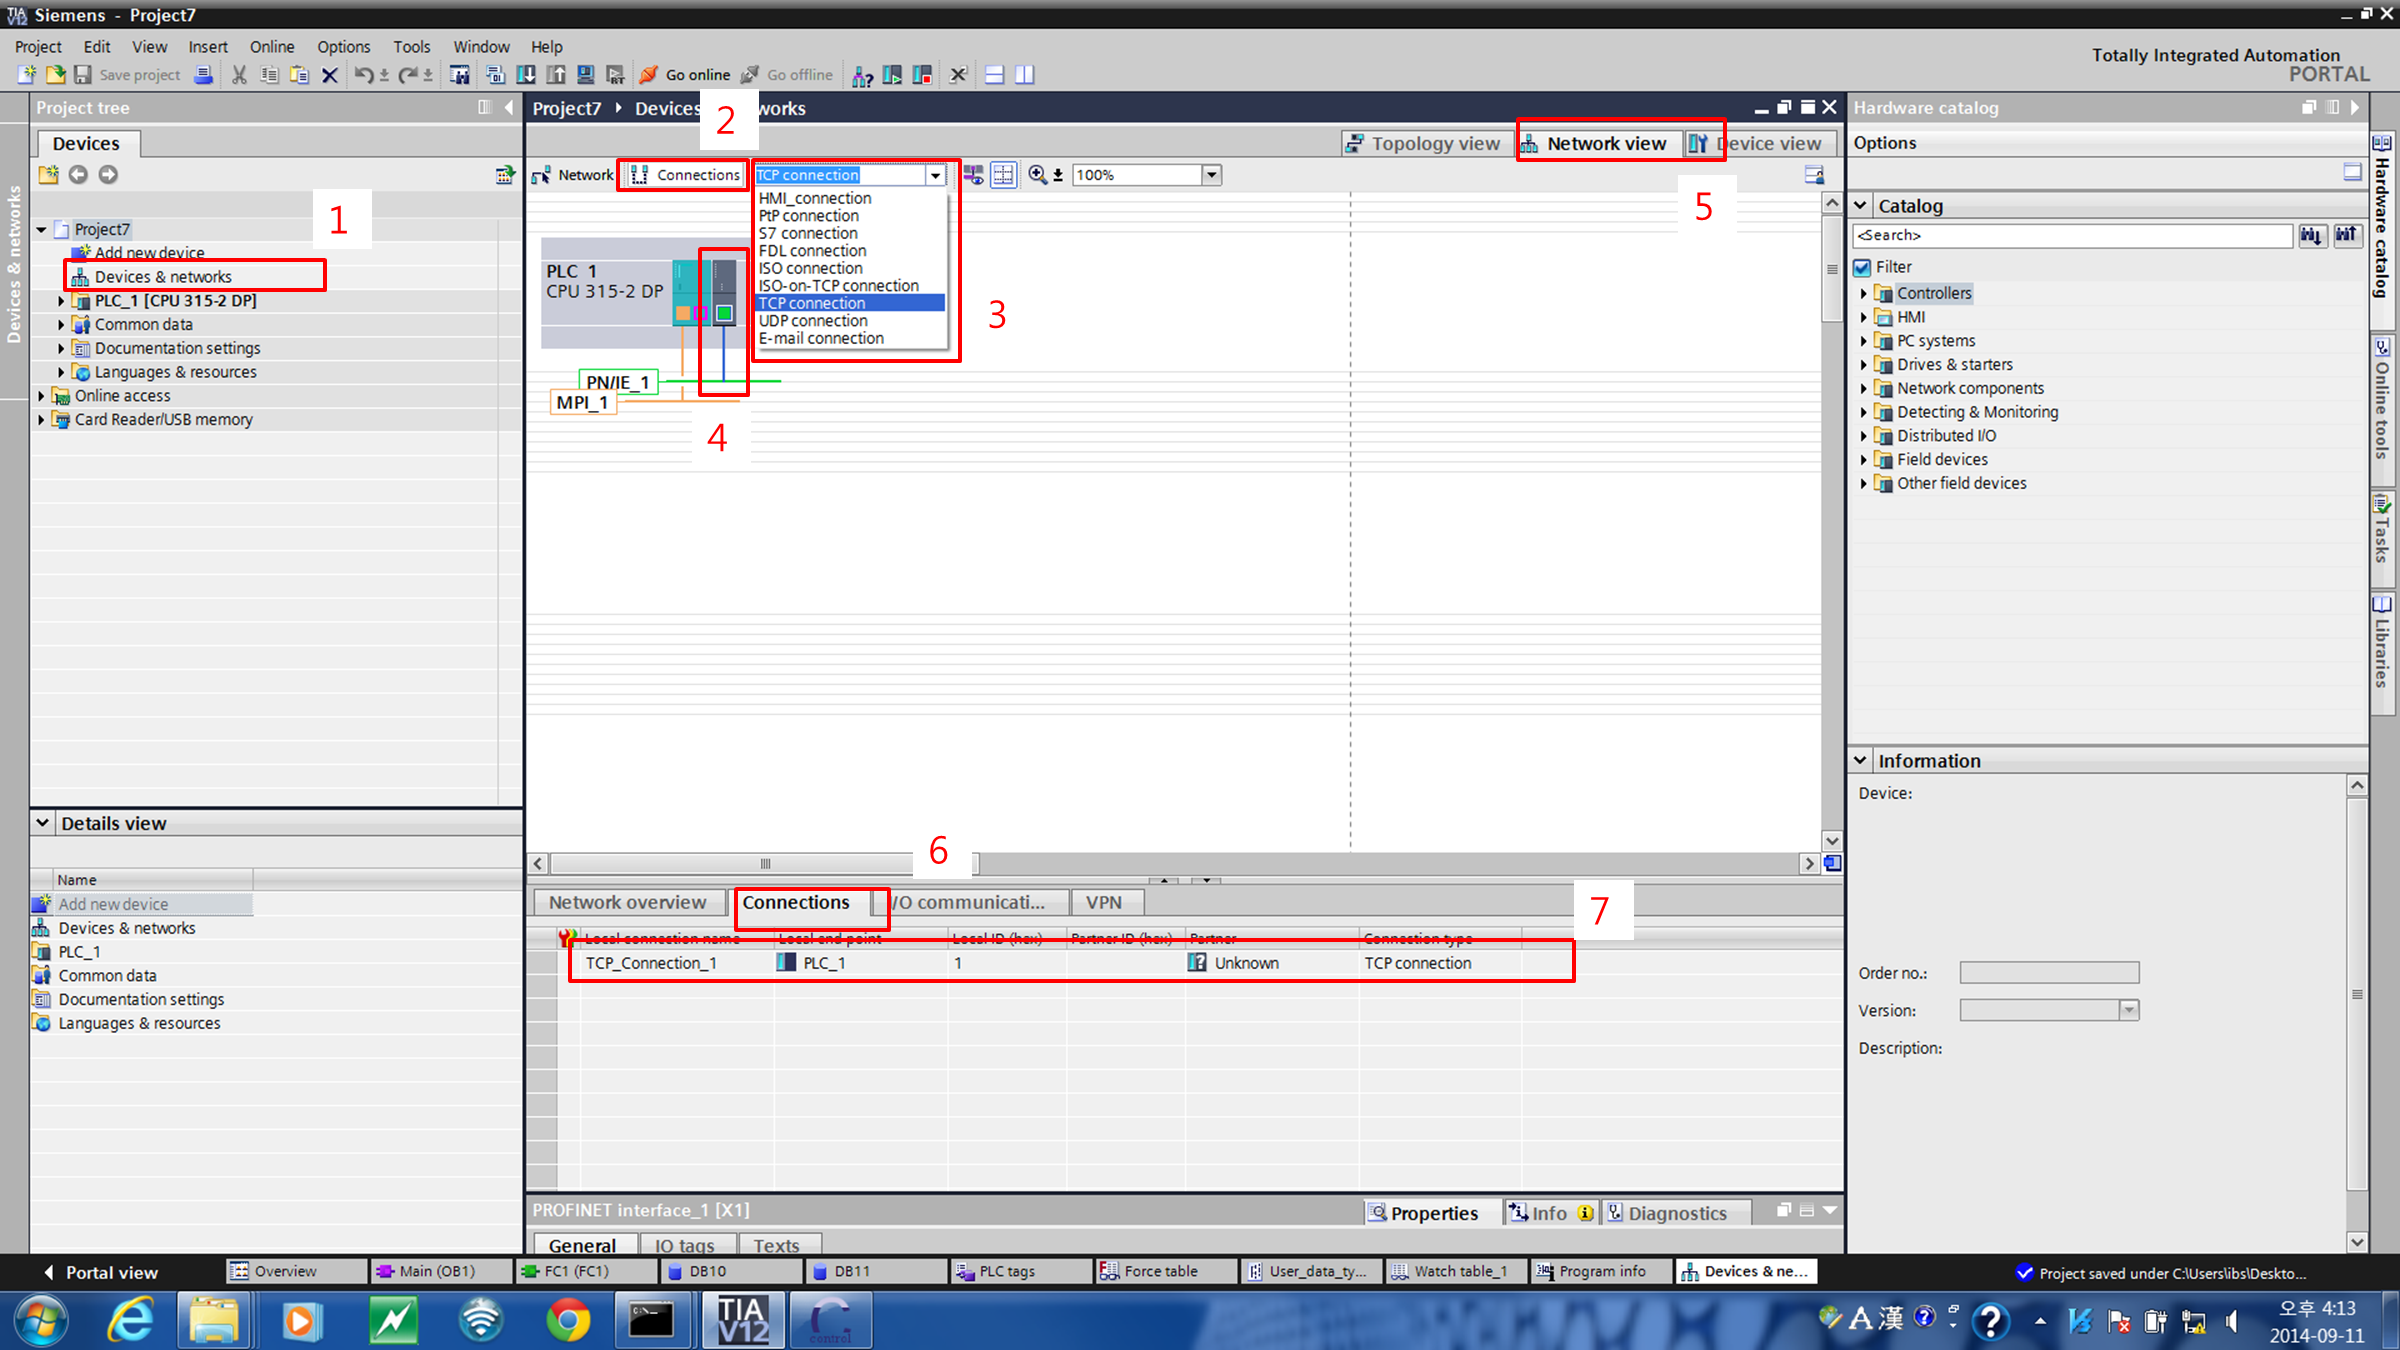
\includegraphics[width=0.96\textwidth]{./images/fig-TCPconnection.png}
  \caption{Connection type configuration}
  \label{}
\end{figure}
\newline Step9. Figure 9 의 1번 박스에 \verb|PN/IE_1|과 \verb|TCP_Connection_1|이 표시된 것을 확인할 수 있을 것이다. 박스 2번의 \verb|Connections| 텝을 클릭하면 \verb|TCP connection|에 관한 상세정보를 확인할 수 있다. 2번 박스의 \verb|TCP_Connection_1|을 선택한 후 하단의 \verb|Properties| 텝의 \verb|General|텝을 클릭하면 박스4번과 같은 Connection 정보창이 나타난다. 여기에서 TCP connection name을 변경할 수 있다. 이 단계에서 중요한 것은 \verb|Connection Path|에서 LOCAL 은 PLC의 통신 모듈로 설정해주고, Partner에 해당하는 부분은 Unknown으로 선택한다. Interface type은 Ethernet으로 설정한다.\\
\begin{figure}[!htb]
  \centering
  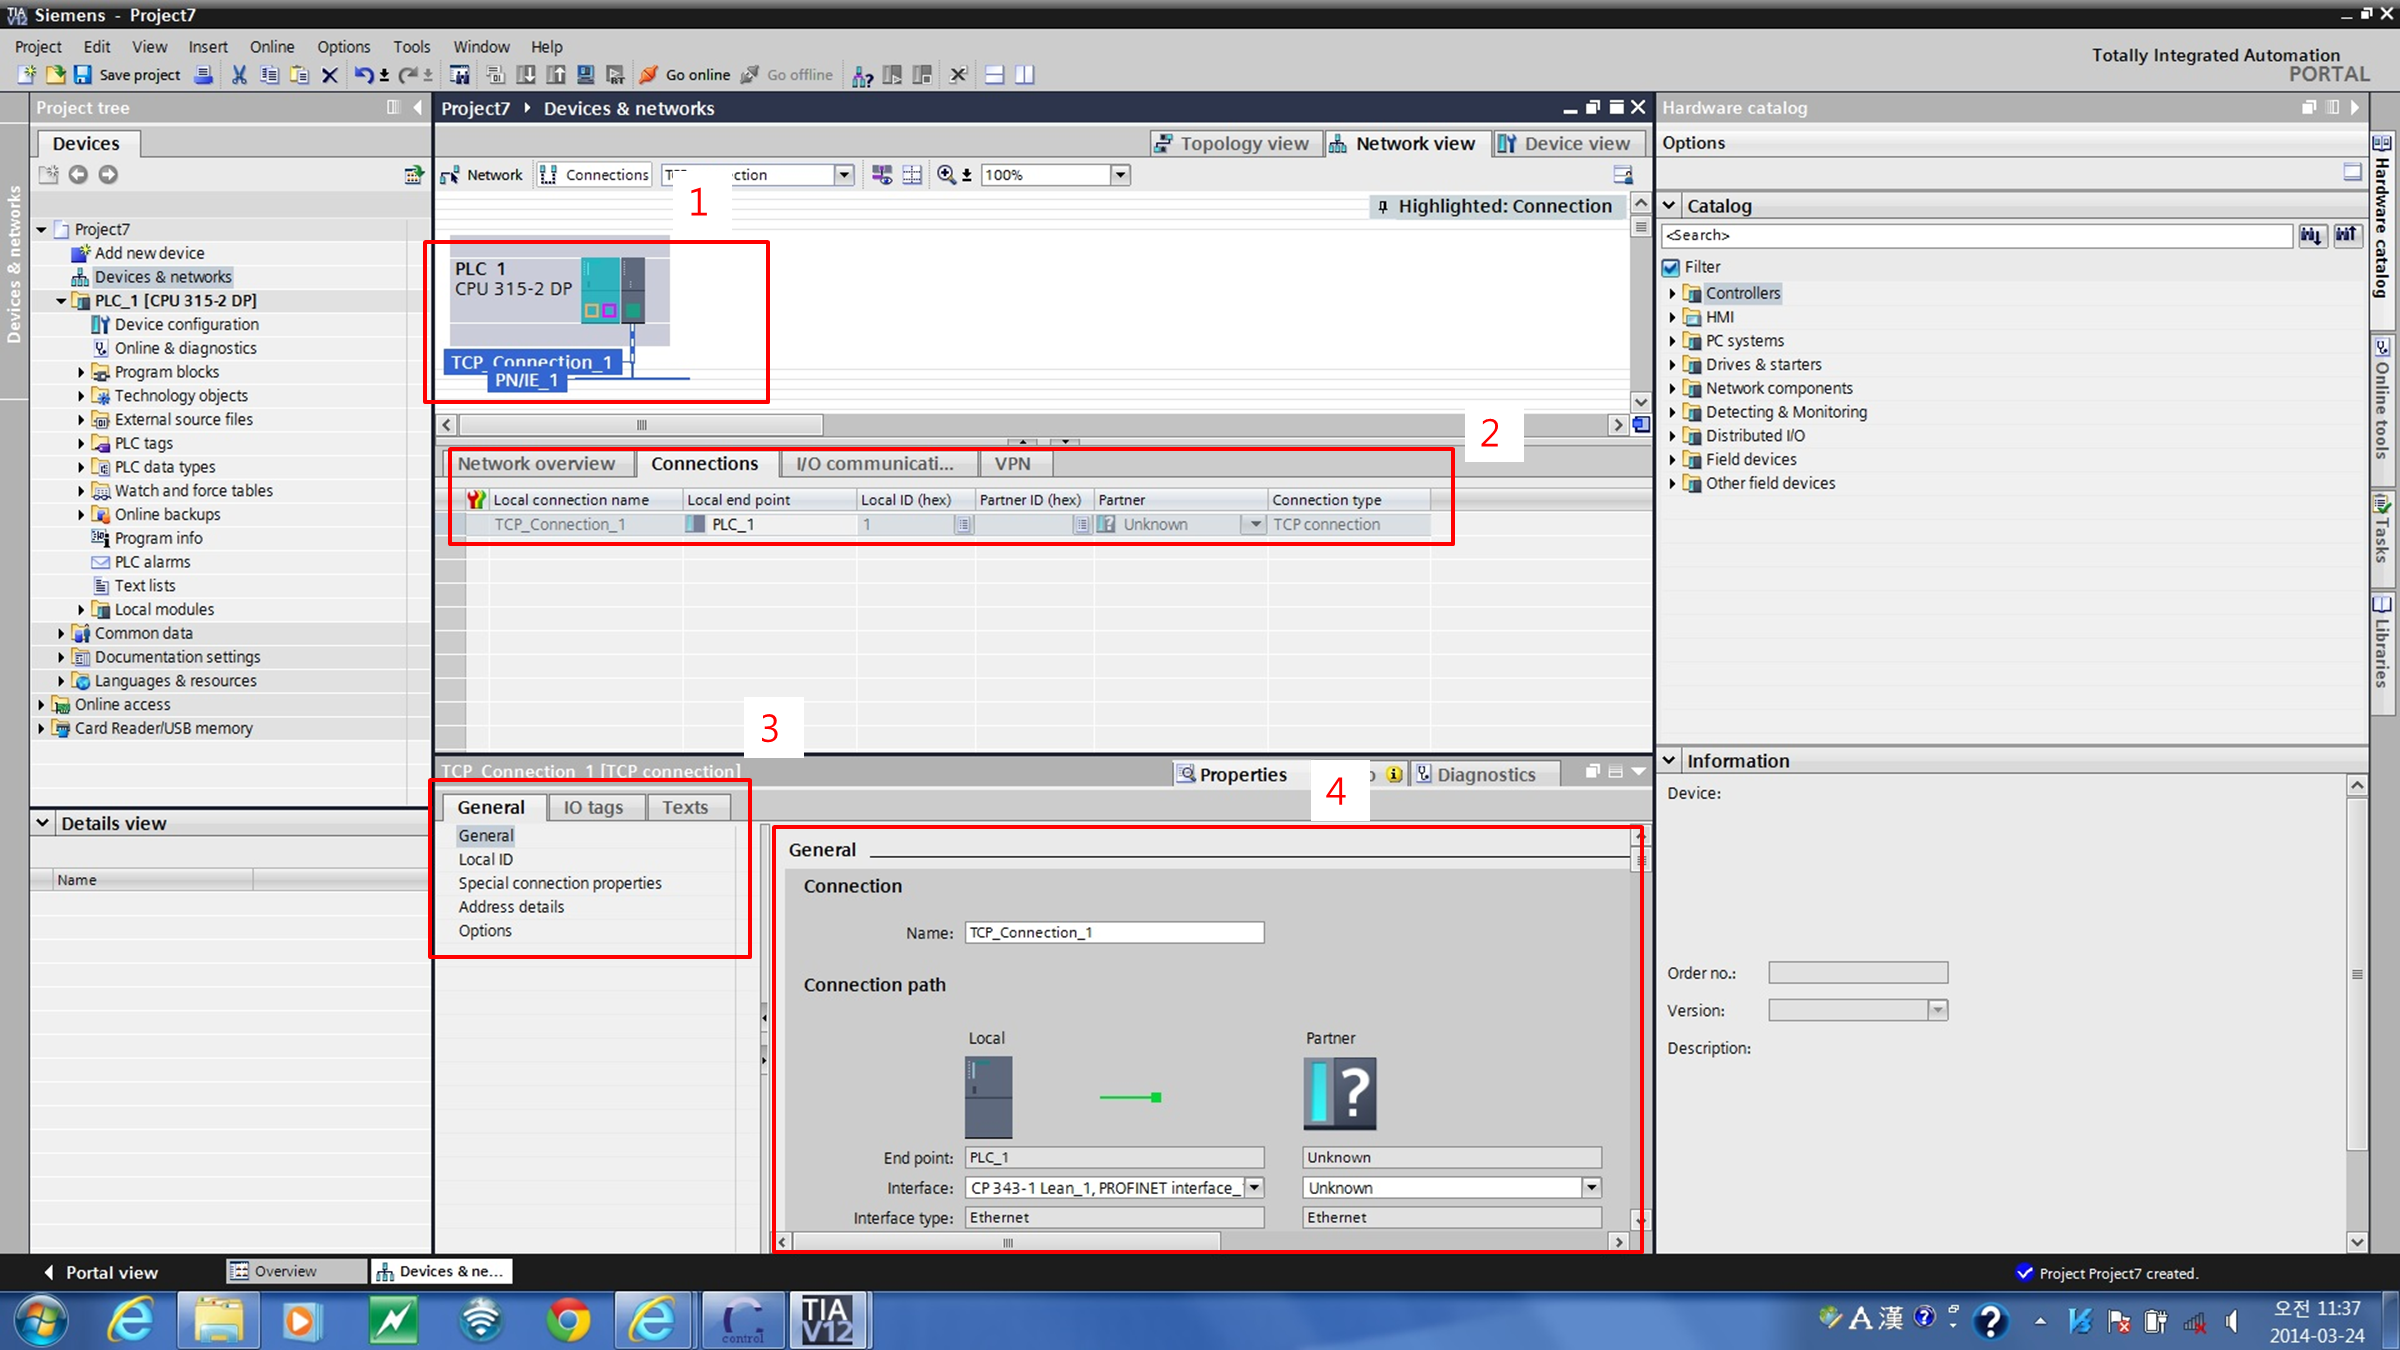
\includegraphics[width=0.96\textwidth]{./images/fig7-local-partner.png}
  \caption{Communication partner configuration}
  \label{}
\end{figure}
\newline Step10. Figure 10 에 설명된 표시된 것과 같이 1번 박스에 해당하는 \verb|General| 텝의 \verb|LocalID| 항목을 클릭하여 3번 박스로 표시된 \verb|Local_ID(hex)| 값과 4번 박스에 표시된 \verb|LADDR| 값을 잘 기록해 둔다. 이 값은 PLC와 EPICS가 통신을 할 때, PLC를 구분하는 고유 정보로 PLC 프로그램작성에서 이용하겠다.\\
\begin{figure}[!htb]
  \centering
  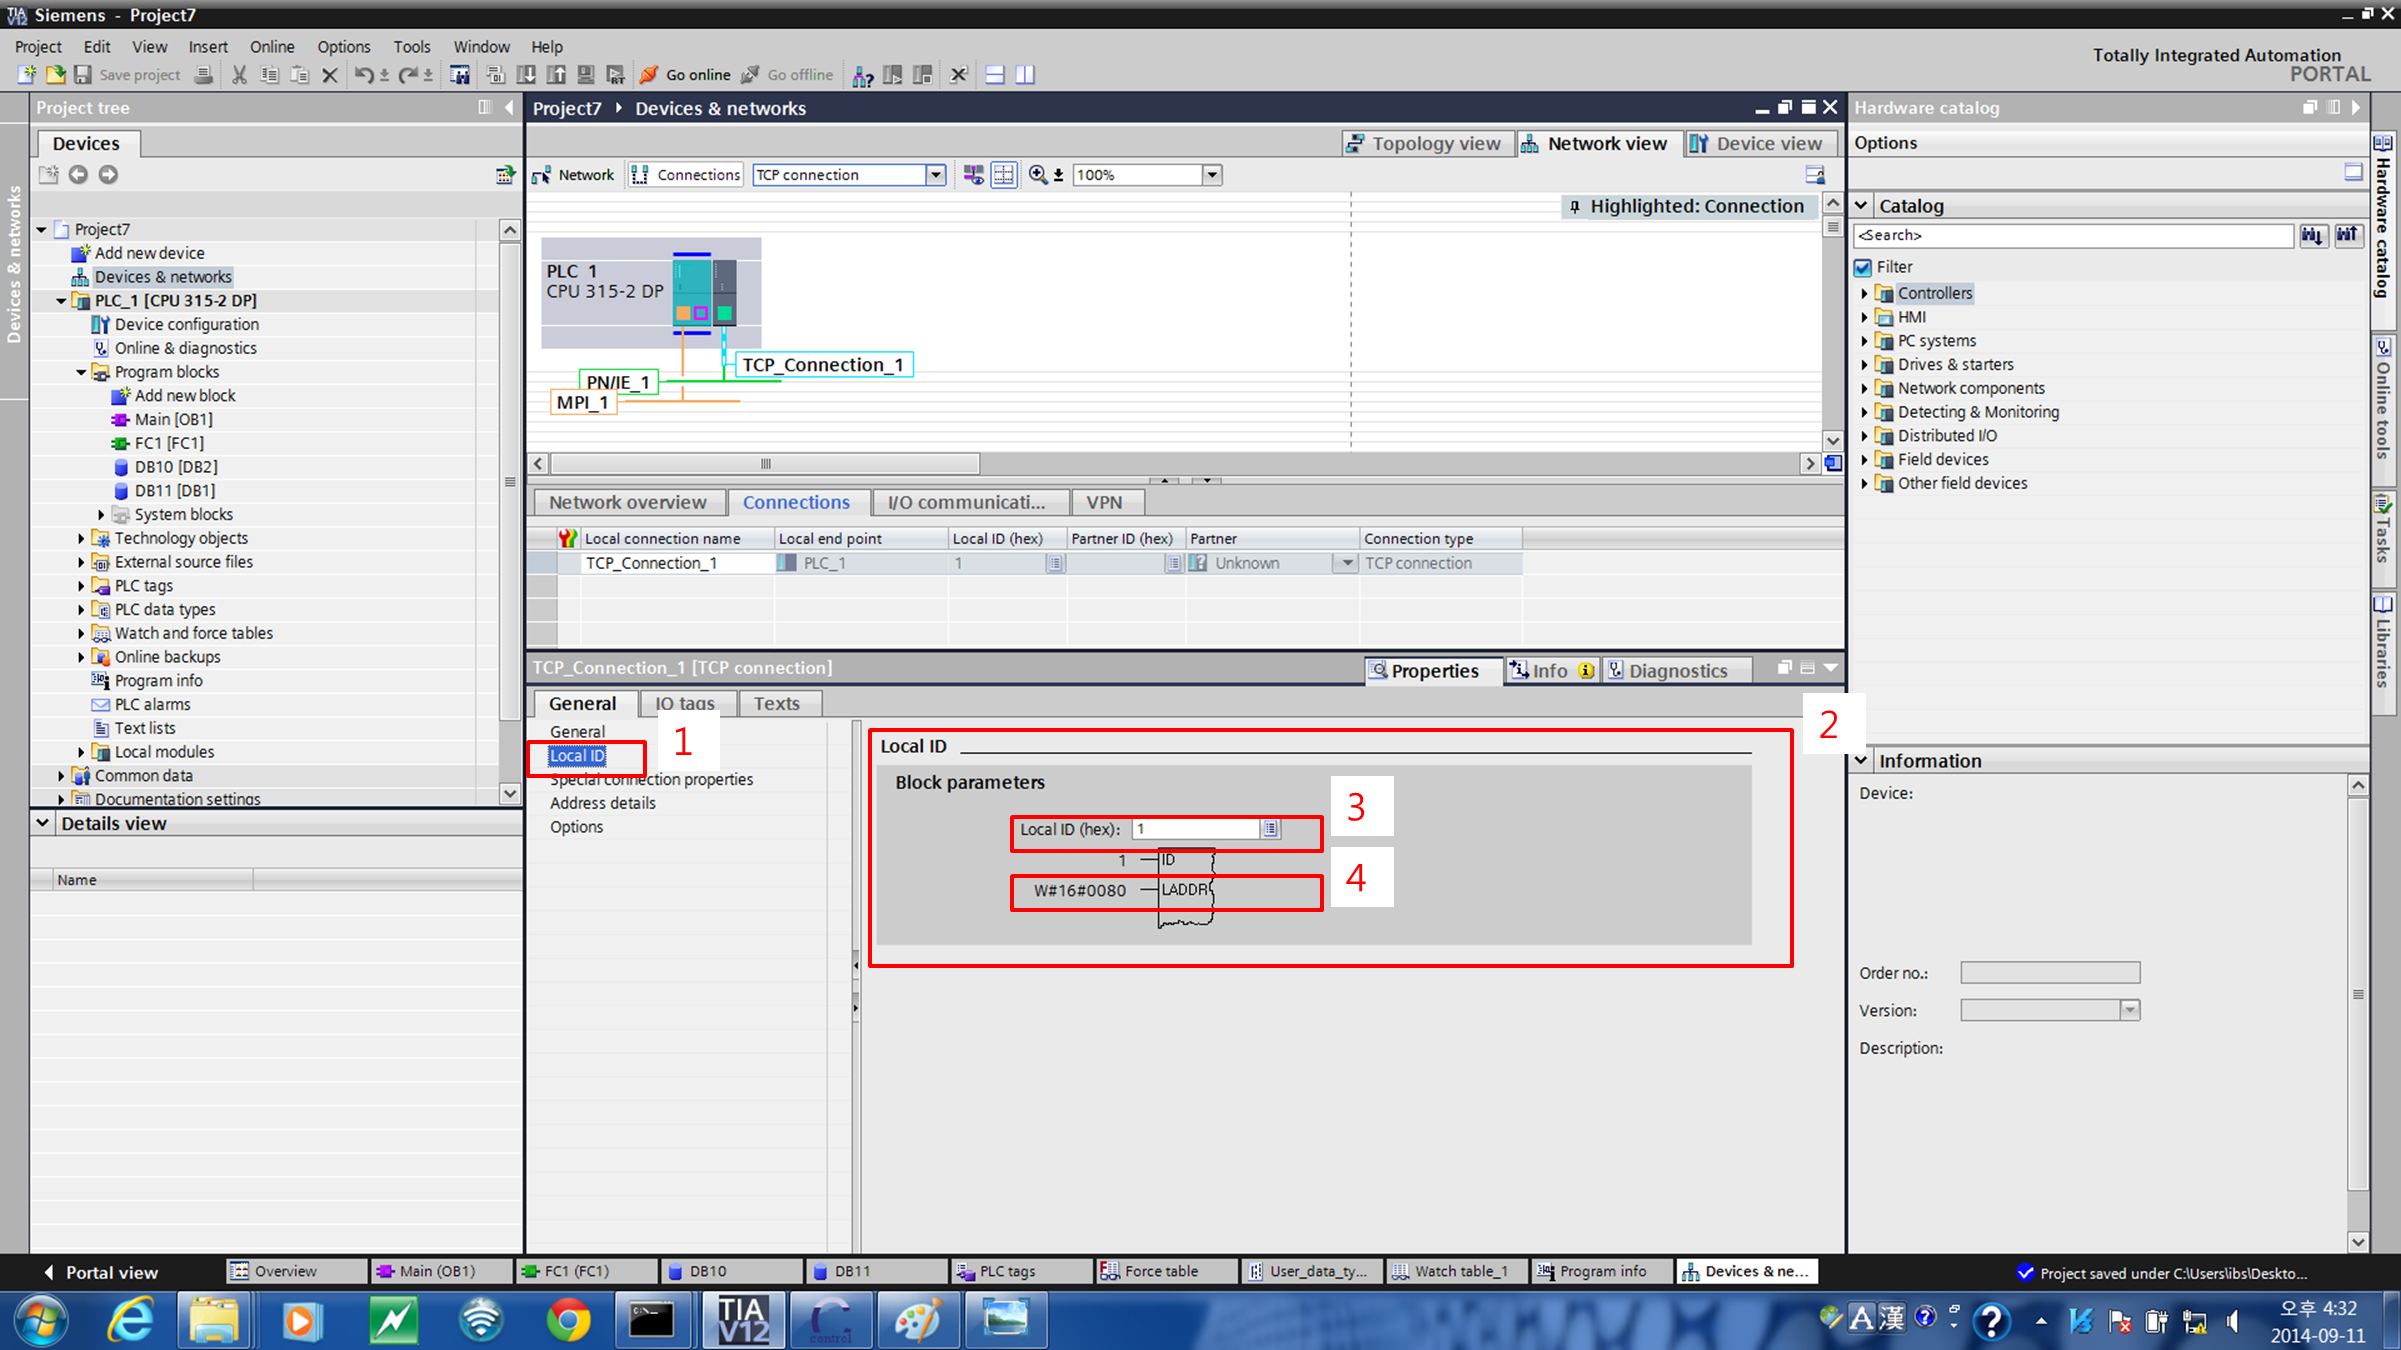
\includegraphics[width=0.96\textwidth]{./images/fig8-localID.png}
  \caption{Check Local ID}
  \label{}
\end{figure}
\newline Step11. 다음 단계로 Figure 11과 같이 \verb|General| 텝의 \verb|Options| 항을 선택하여 2번 박스에 표시된 내용과같이 Mode값을 SEND/RECEIVE로 선택한다. Mode 값은 어떤 방식으로 데이타 패킷을 주고 받을 것인지를 지정해주는 부분이다. 여기까지 설정하였다면 EPICS와의 통신을 위한 CP 모듈의 설정이 모두 끝났다.
\begin{figure}[!htb]
  \centering
  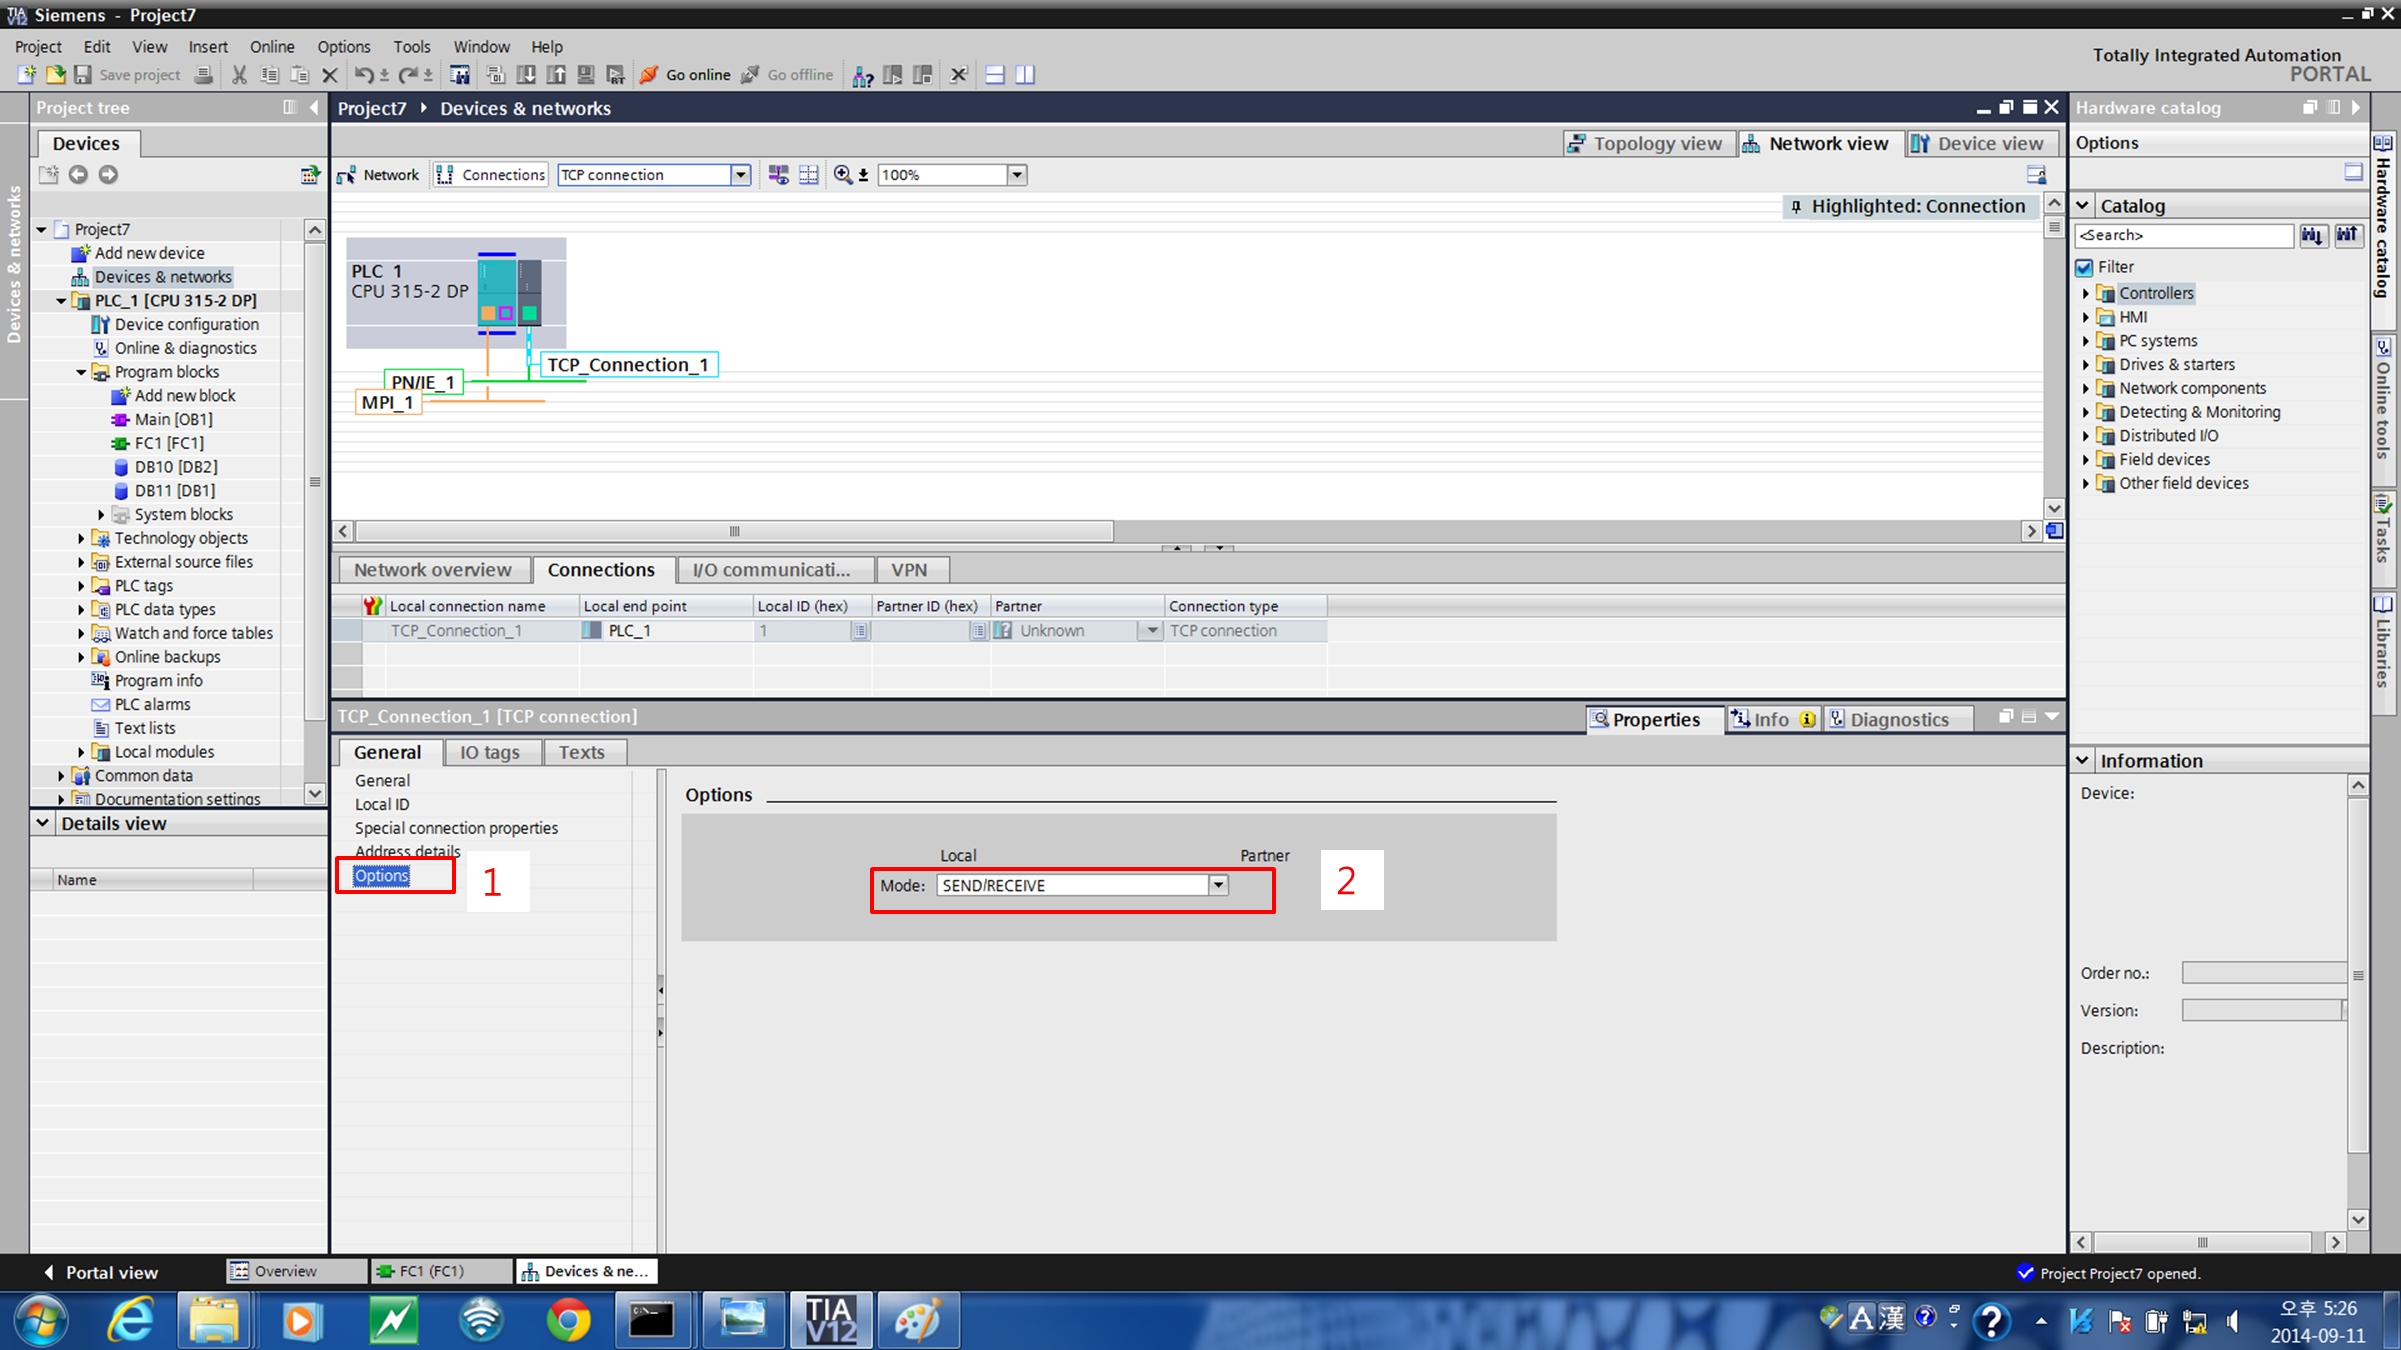
\includegraphics[width=0.96\textwidth]{./images/fig9-options.png}
  \caption{Data exchange mode configuration}
  \label{}
\end{figure}
\newline Step12. CPU 및 Power supplier 그리고 CP 모듈까지 설정하였고, 이제 입출력 모듈을 각각의 순서에 해당하는 slot에 설정한다. 설정 방법은 Power supplier 모듈의 설정 방법과 동일한 방법으로 진행한다. 모든 모듈을 설정하였으면 설정한 모듈 정보를 확인하고, 입출력 모듈의 경우 I address와 Q address 주소를 Figure 12 의 4번 박스에서 확인한다. 
\begin{figure}[!htb]
  \centering
  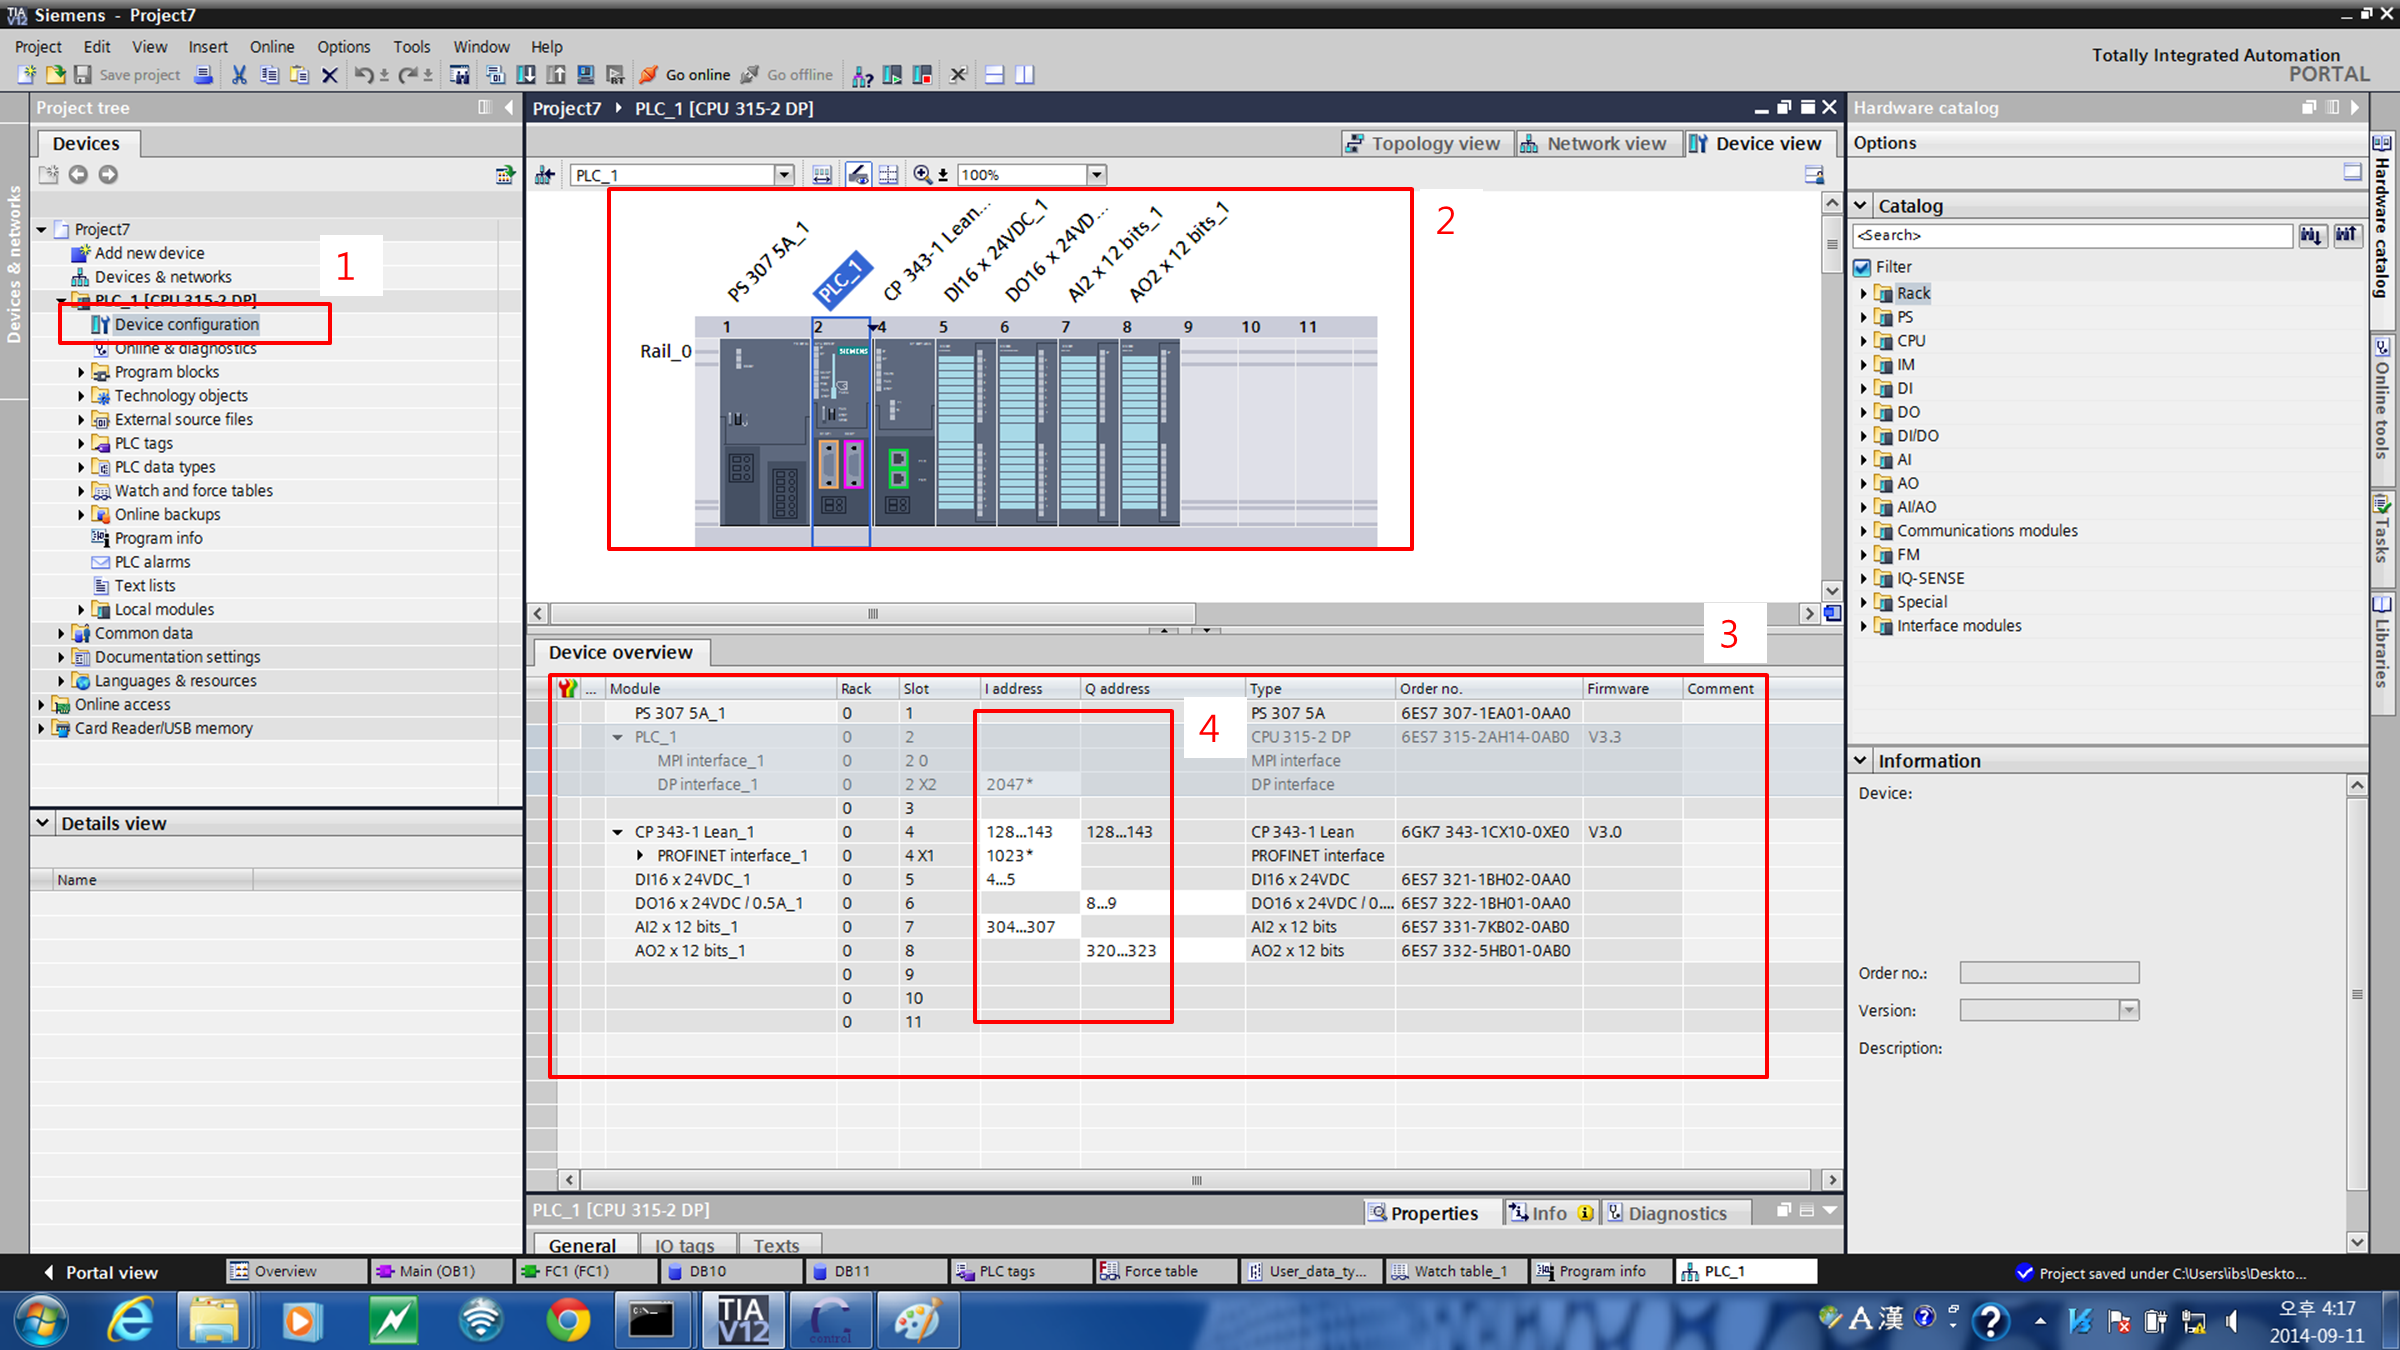
\includegraphics[width=0.96\textwidth]{./images/fig10-device-configuration.png}
  \caption{Input, output module configuration}
  \label{}
\end{figure}
\newline 자동으로 할당된 입출력 주소는 다음과 같음을 확인할 수 있다.
\begin{itemize}
\item Digital Input 에 해단하는 I address : 4-5 
\item Digital Output 에 해당하는 Q address : 8-9
\item Analog Input 에 해당하는 I address : 304-307
\item Analog Output 에 해당하는 Q address : 320-323 
\end{itemize}
Step13. FIgure 13 의 1번 박스의 \verb|Compile and Download|를 클릭하고 나서 2번 박스의 \verb|Type of the PG/PC interface| 값을 MPI로 선택하고 \verb|Load|를 클릭하면 PLC 설정에 대한 내용을 PLC로 다운로드하고, PLC가 설정대로 동작하게 된다. 이후부터는 다운로드시 \verb|Type of the PG/PC interface|를 \verb|PN/IE|로 선택할 수 있다. \verb|PN/IE|로 선택할 경우 MPI 케이블을 제거하여도 네트워크를 통해서 다운로드가 된다. 
\begin{figure}[!htb]
  \centering
  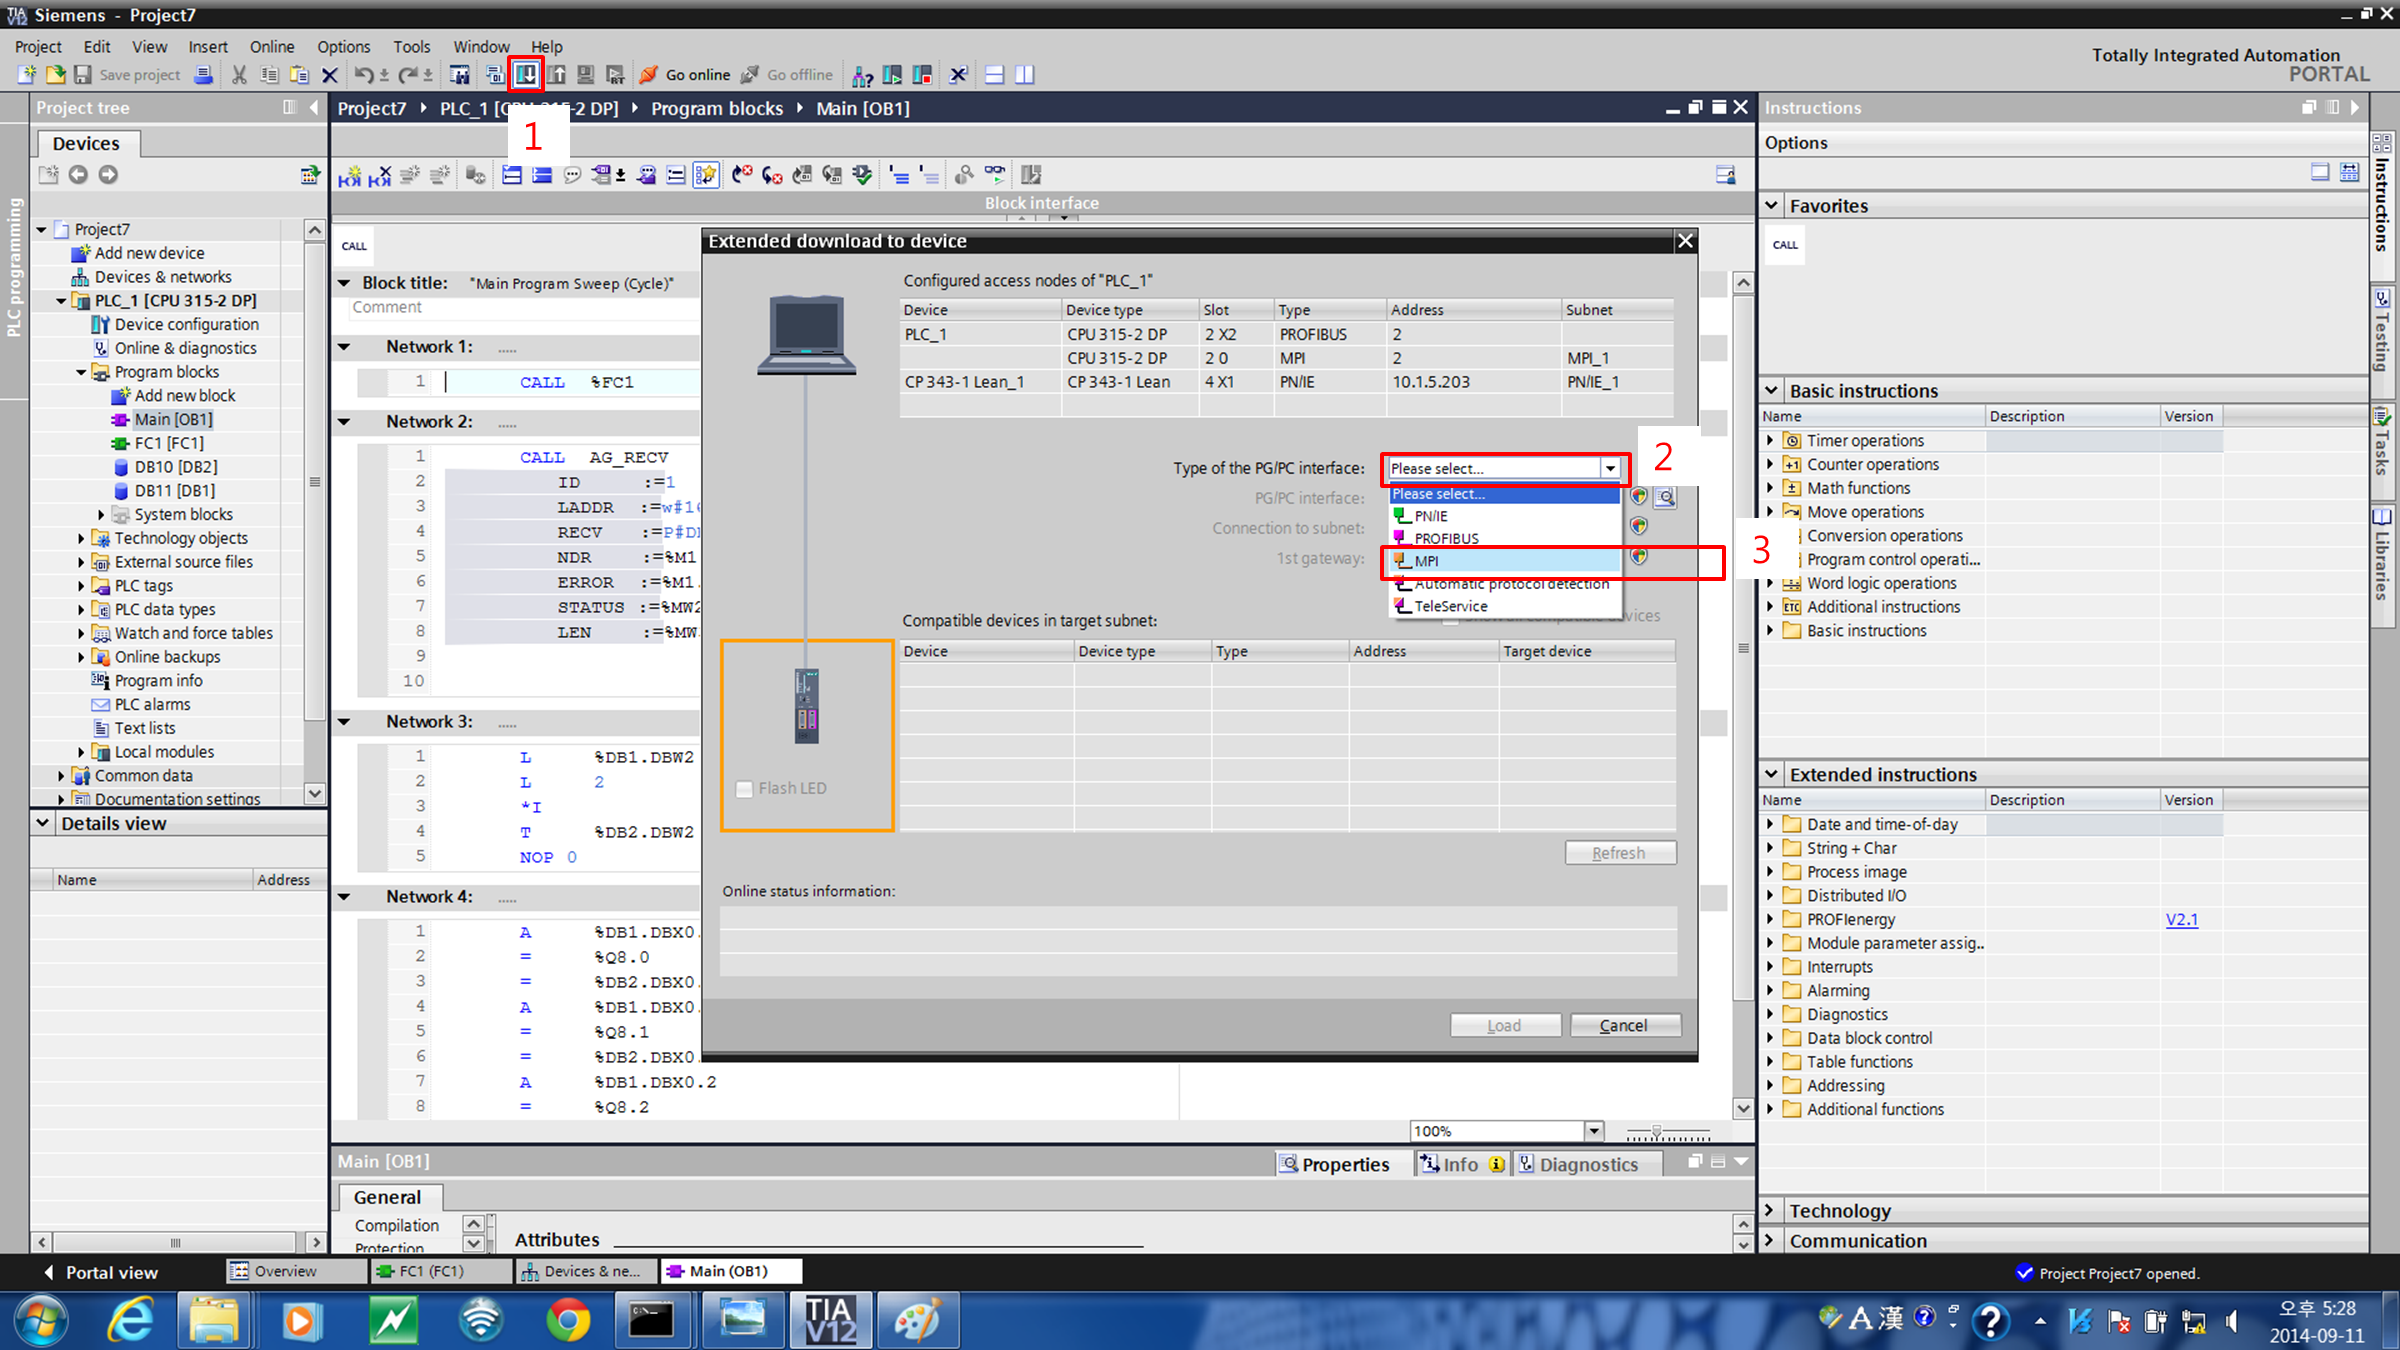
\includegraphics[width=0.96\textwidth]{./images/fig-MPI.png}
  \caption{Hardware configuration download}
  \label{}
\end{figure}


\section{PLC Programming}
PLC는 일반적으로 Ladder Diagram이라는 언어를 이용하여 프로그래밍 하지만 이 외에도 다양한 형태의 언어들을 사용할 수 있으며, PLC Vendor마다 조금씩 차이가 있다. 여기에서는 STL(Statement List)라는 언어를 이용하겠다. \\
\newline  PLC 프로그램은 Main[OB1] 블락으로부터 시작되며, FC1 함수 블락을 호출한다. 또한 시스템 블락인 \verb|AG_SEND|와 \verb|AG_RECV|를 이용하여 데이타를 주고받게된다.\\
 실제 프로그램의 내용과 순서는 다음과 같다.\\
\newline Step1. Figure 14 의 1번 박스에 있는 \verb|Program Blocks|를 틀릭하면 \verb|Add blocks|와 \verb|Main[OB1]|이라는 프로그램 블락이 나타난다. 이 프로그램 블락은 C/C++와 같은 프로그래밍 언어에서 함수와 같은 기능을 한다고 생각하면 된다.\\
\newline  우리는 EPICS로부터 데이타를 받아들이는 데이타 블락과 EPICS로 보내기 위한 데이타 블락, 준비된 데이터 블락을 EPICS로부터 받아들이는 함수 블락, EPICS로 내보내는 함수 블락이 필요하다.이들을 추가하기 위해서 \verb|Add block|을 클릭한다.\\
\begin{figure}[!htb]
  \centering
  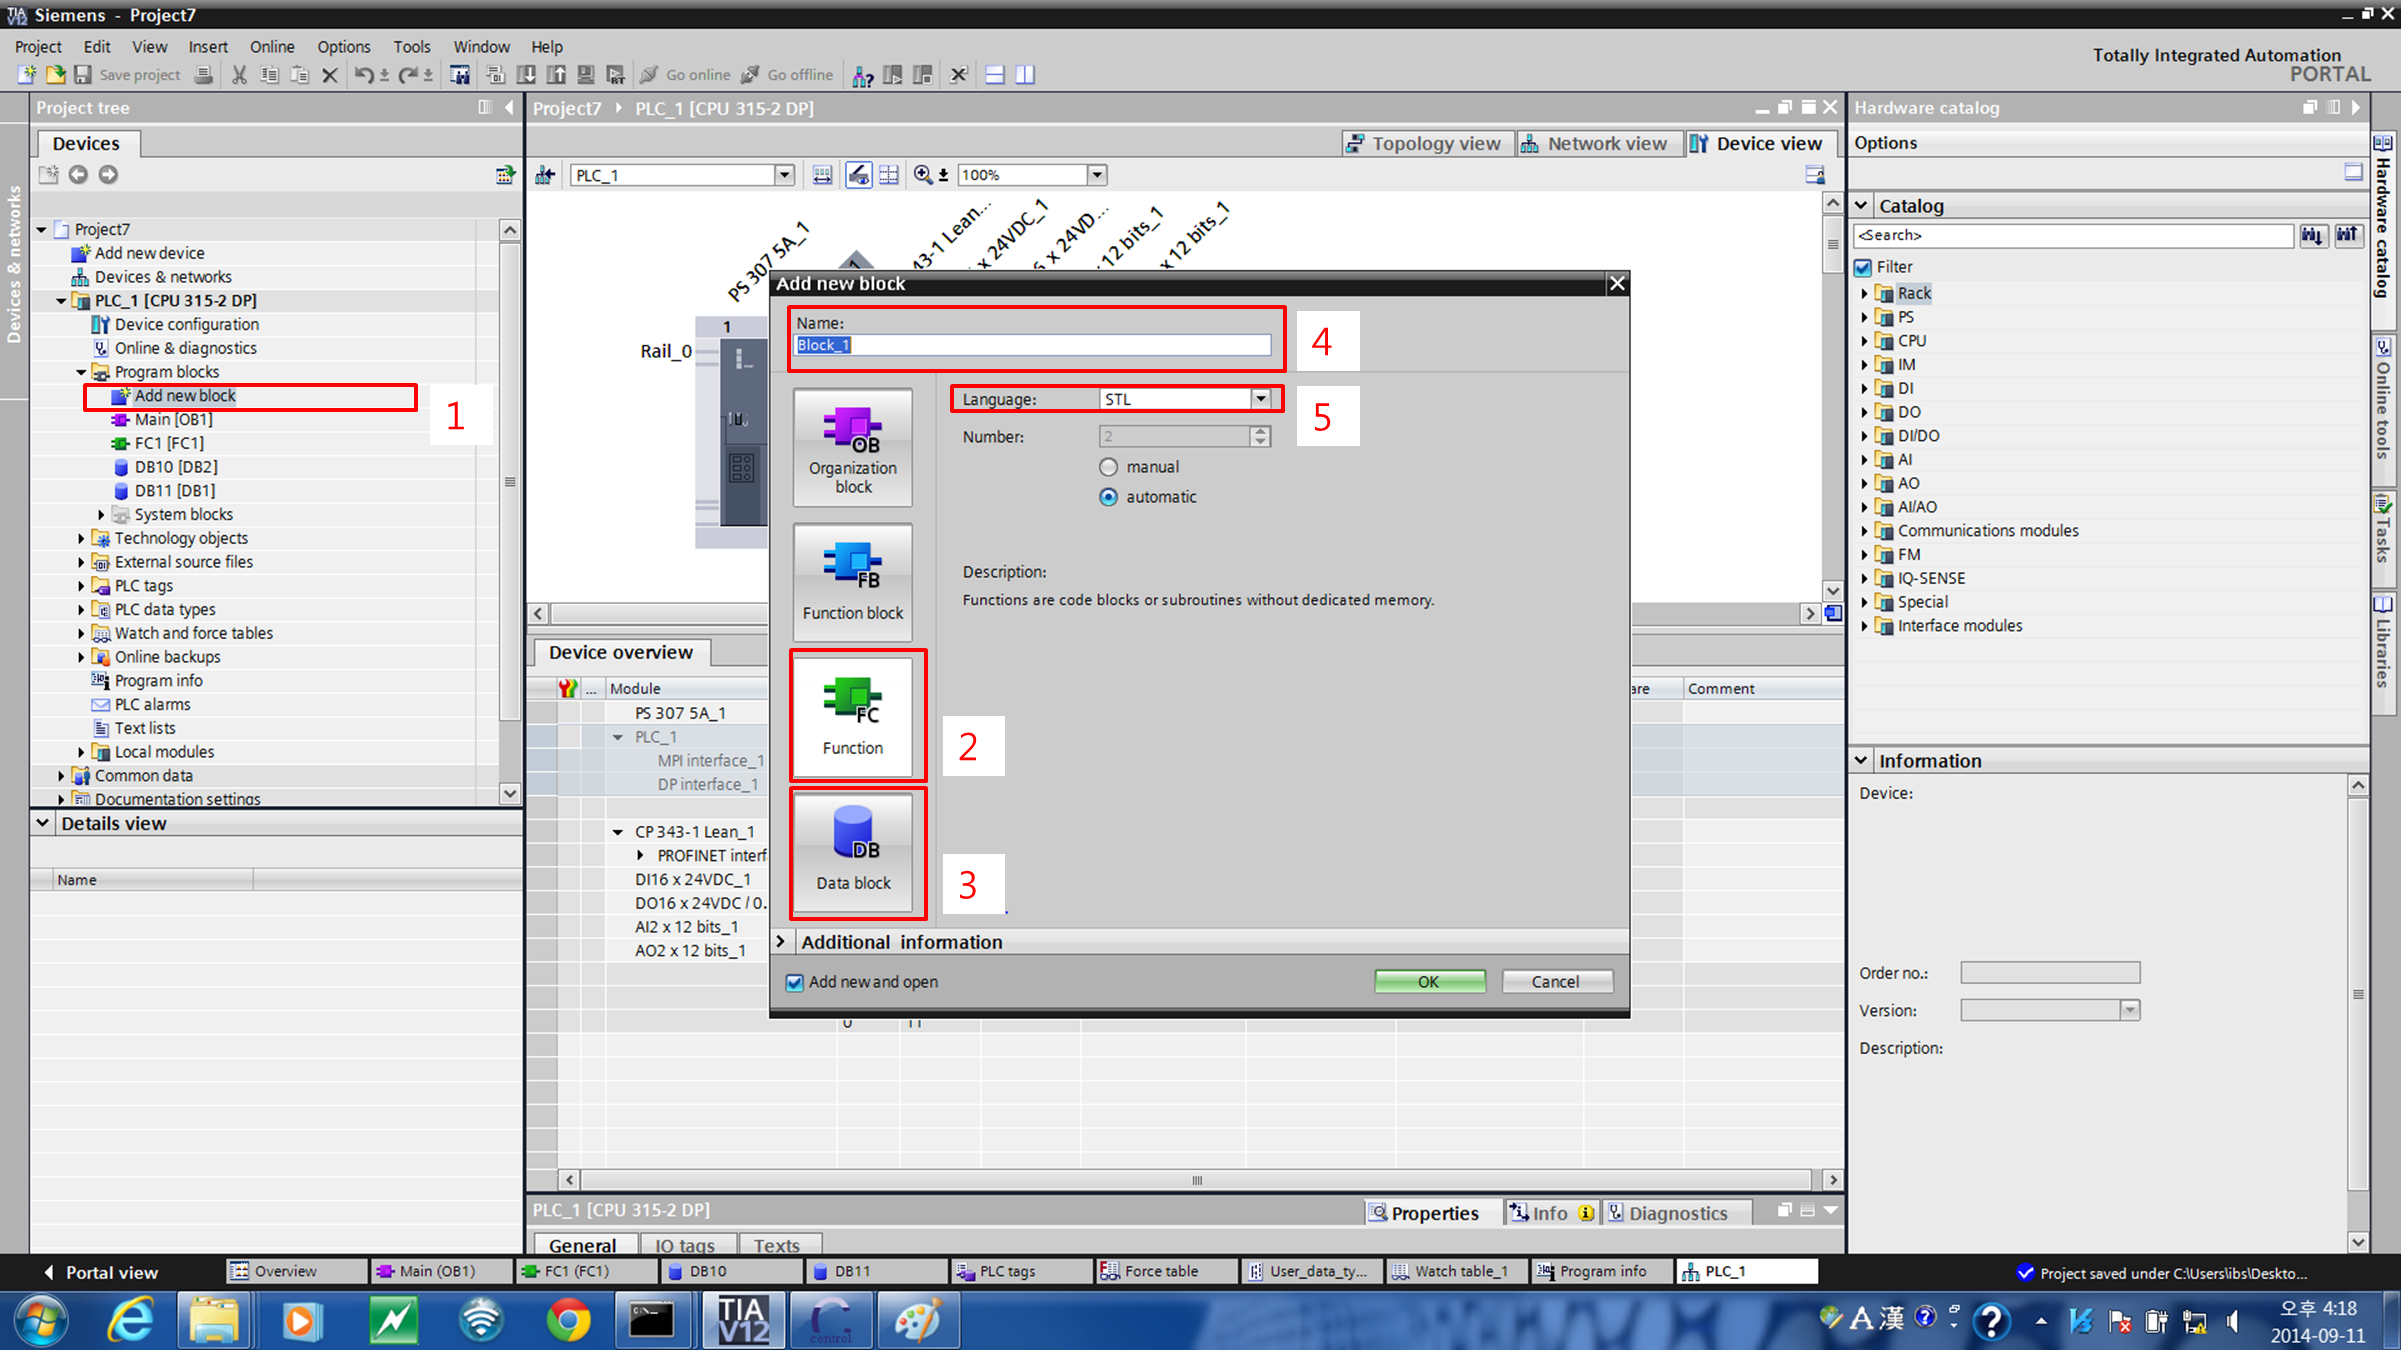
\includegraphics[width=0.96\textwidth]{./images/fig11-FCblock.png}
  \caption{Add function block}
  \label{}
\end{figure}
\newline Step2. Figure 15 의 2번 박스를 클릭하여 함수 블럭을 하나 생성하고 4번 박스에 FC1이라는 이름을 주고, 5번 박스를 클릭하여 언어를 STL로 선택한 후 \verb|OK|를 클릭하여 생성한다. 
\newline 또, 두개의 데이타 블락이 필요하므로 박스3번의 \verb|DB, Datablock|를 클릭하여 DB10이라는 이름을 부여하고, Type에 Global DB를 선택한다.같은 방법으로 DB11을 생성한다.\\
\begin{figure}[!htb]
  \centering
  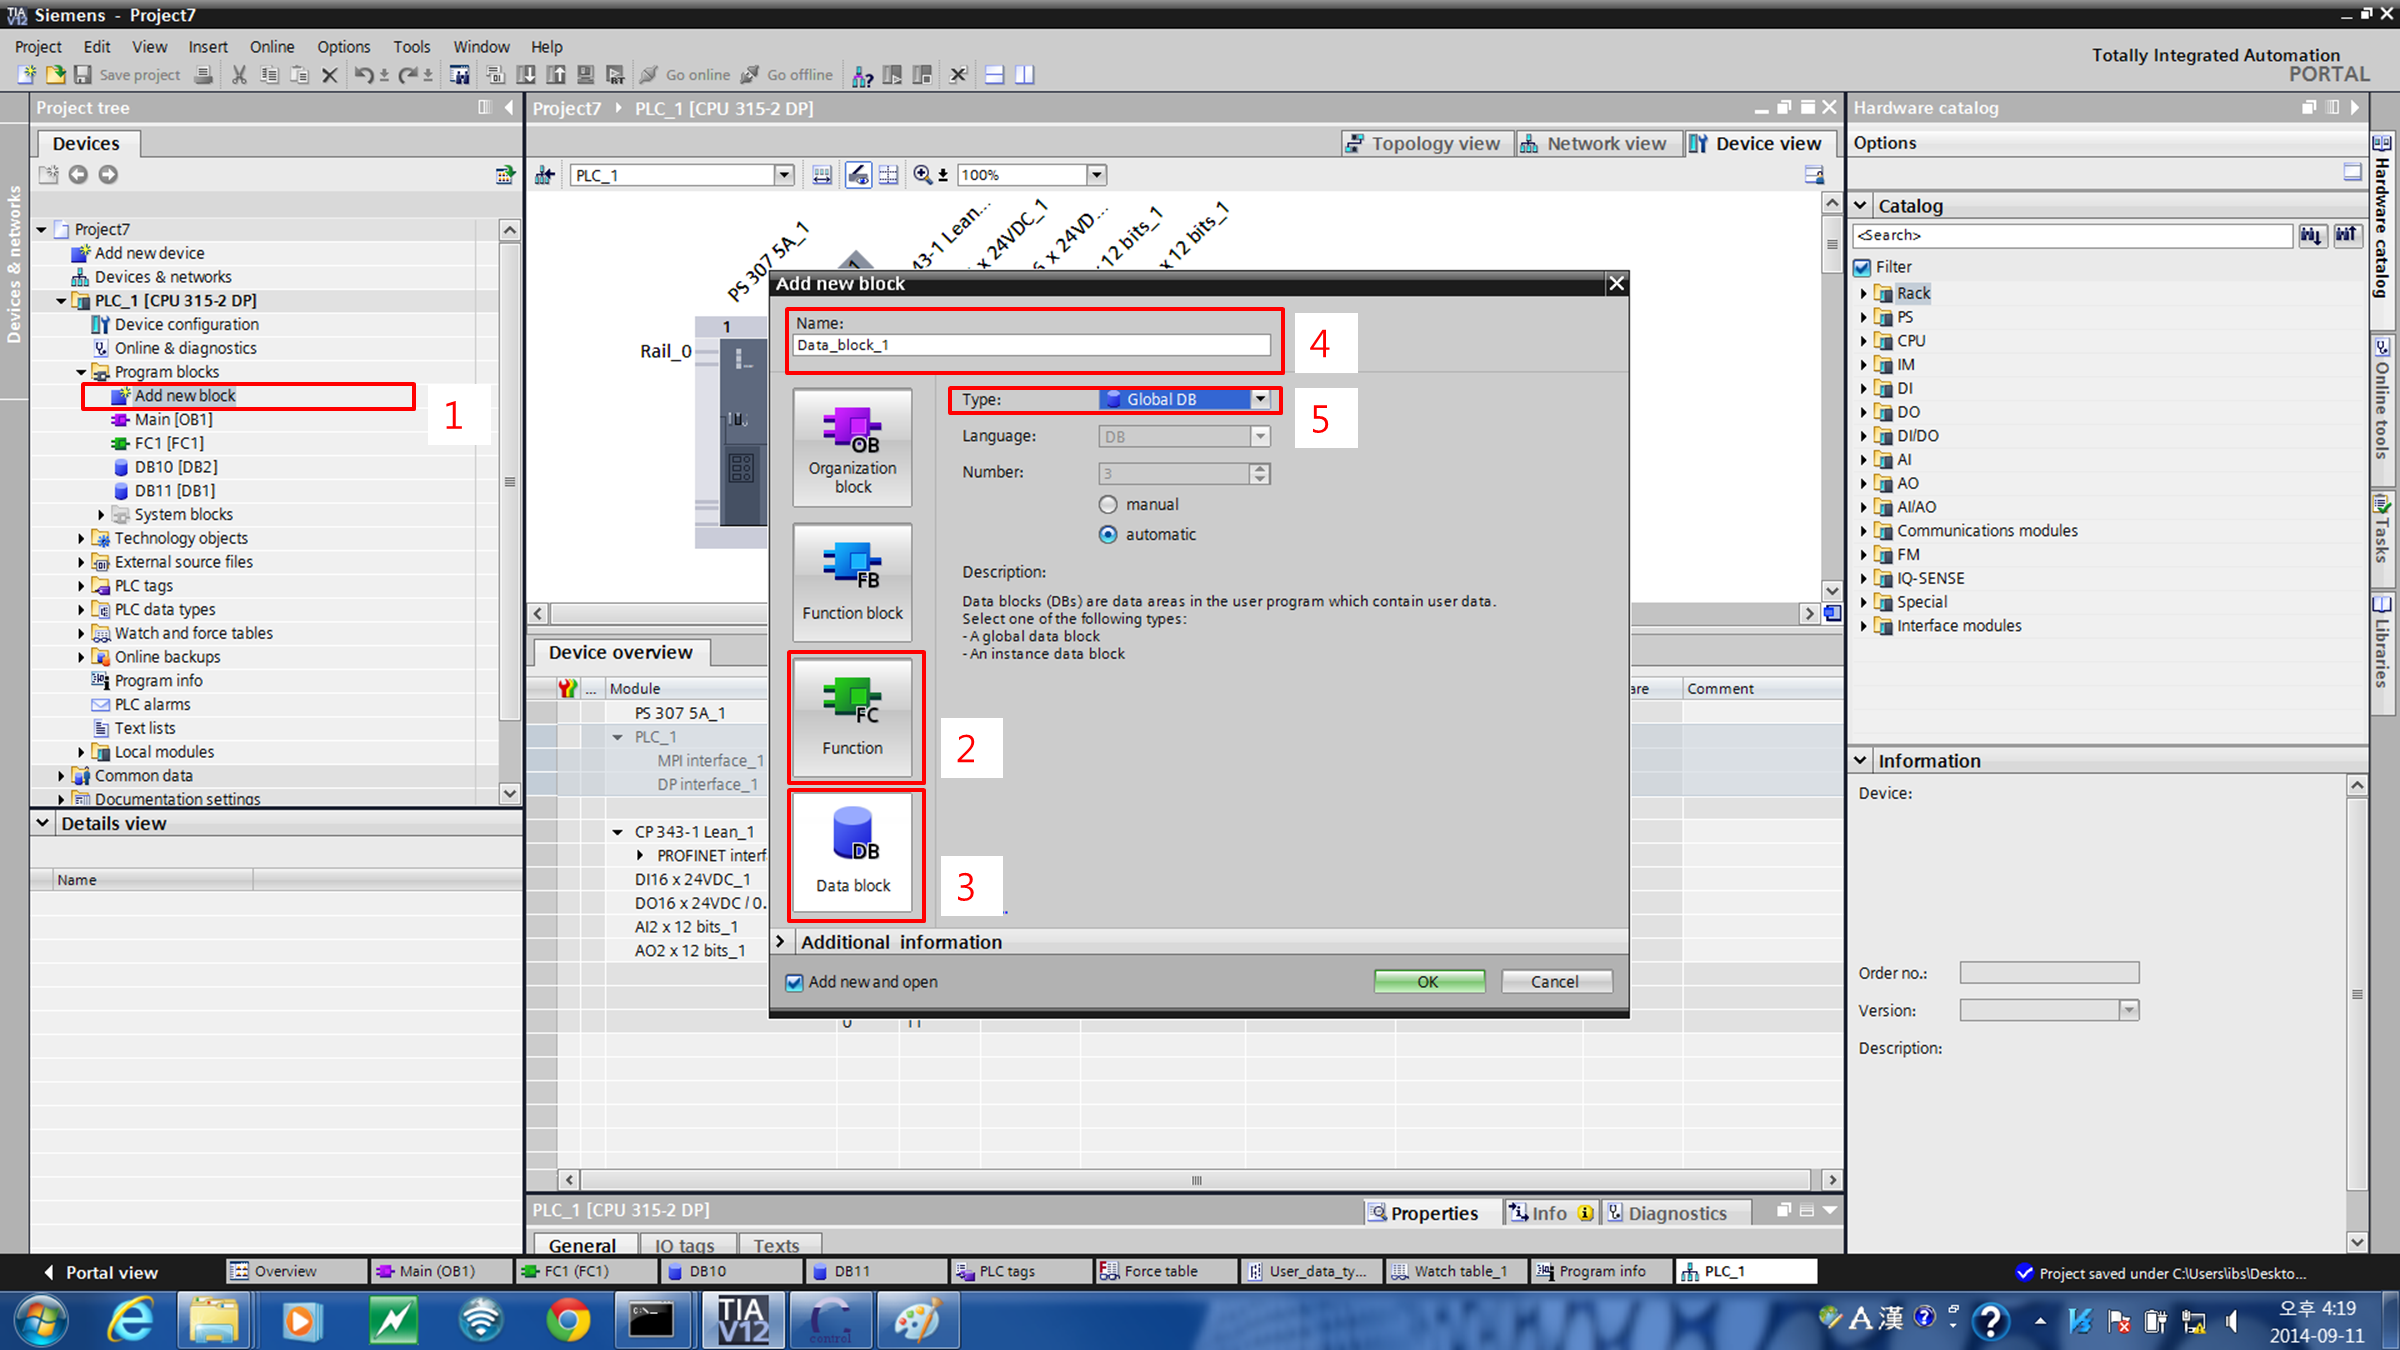
\includegraphics[width=0.96\textwidth]{./images/fig-DBblock.png}
  \caption{Add data block}
  \label{}
\end{figure}
\newline Step3. Figure 16 의 박스 1 \verb|Main[OB1]| 을 클릭하여 다음과 같은 프로그램을 작성한다.\\
\begin{figure}[!htb]
  \centering
  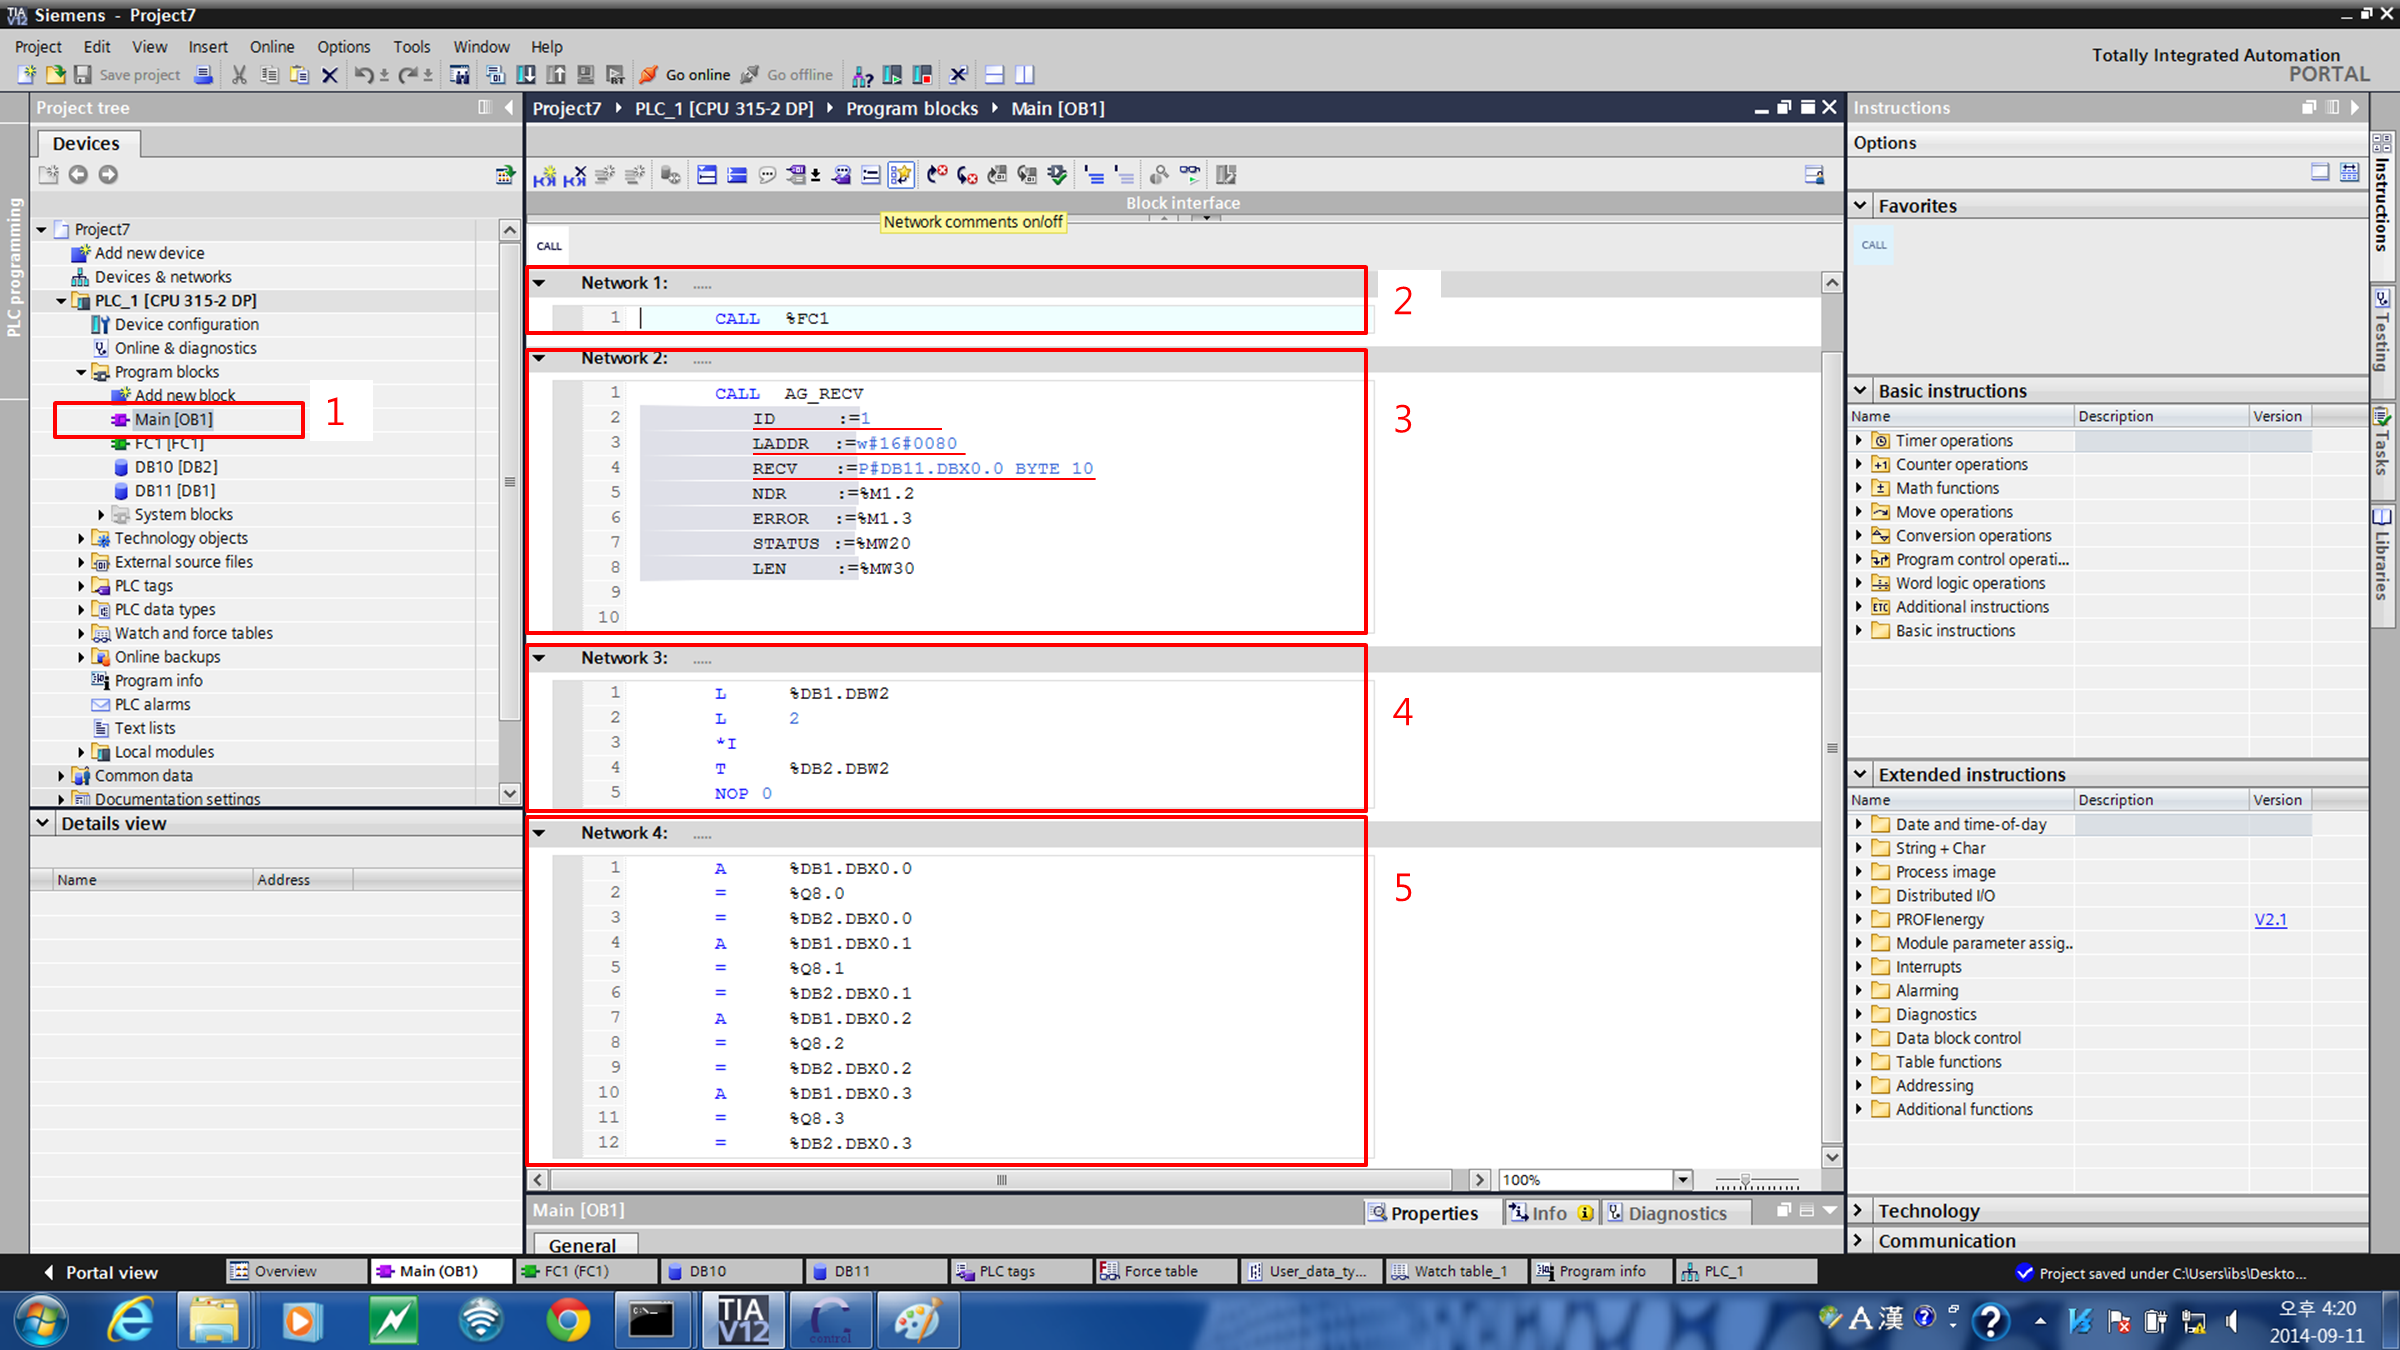
\includegraphics[width=0.96\textwidth]{./images/fig12-main.png}
  \caption{Main program source code}
  \label{}
\end{figure}
\begin{lstlisting}[style=termstyle]
Network1:
	CALL "FC1"

Network2:
	CALL AG_RECV
	ID	:=1
	LADDR	:=w#16#0080
	RECV	:=P#DB11.DBX0.0 BYTE 10
	NDR	:=%M1.2
	ERROR	:=%M1.3
	STATUS	:=%MW20
	LEN	:=%MW30

Network3:
	L	%DB.DBW2
	L	2
	*I
	T	%DB2.DBW2
	NOP	0

Network4:
	A	%DB1.DBX0.0
	=	%Q8.0
	=	%DB2.DBX0.0
	A	%DB1.DBX0.1
	=	%Q8.1
	=	%DB2.DBX0.1
	A	%DB1.DBX0.2
	=	%Q8.2
	=	%DB2.DBX0.2
	A	%DB1.DBX0.3
	=	%Q8.3
	=	%DB2.DB0.3
\end{lstlisting}
Step4. \verb|FC1|함수를 더블 클릭하여 Figure 17 같이 내용을 추가한다.\\
\begin{figure}[!htb]
  \centering
  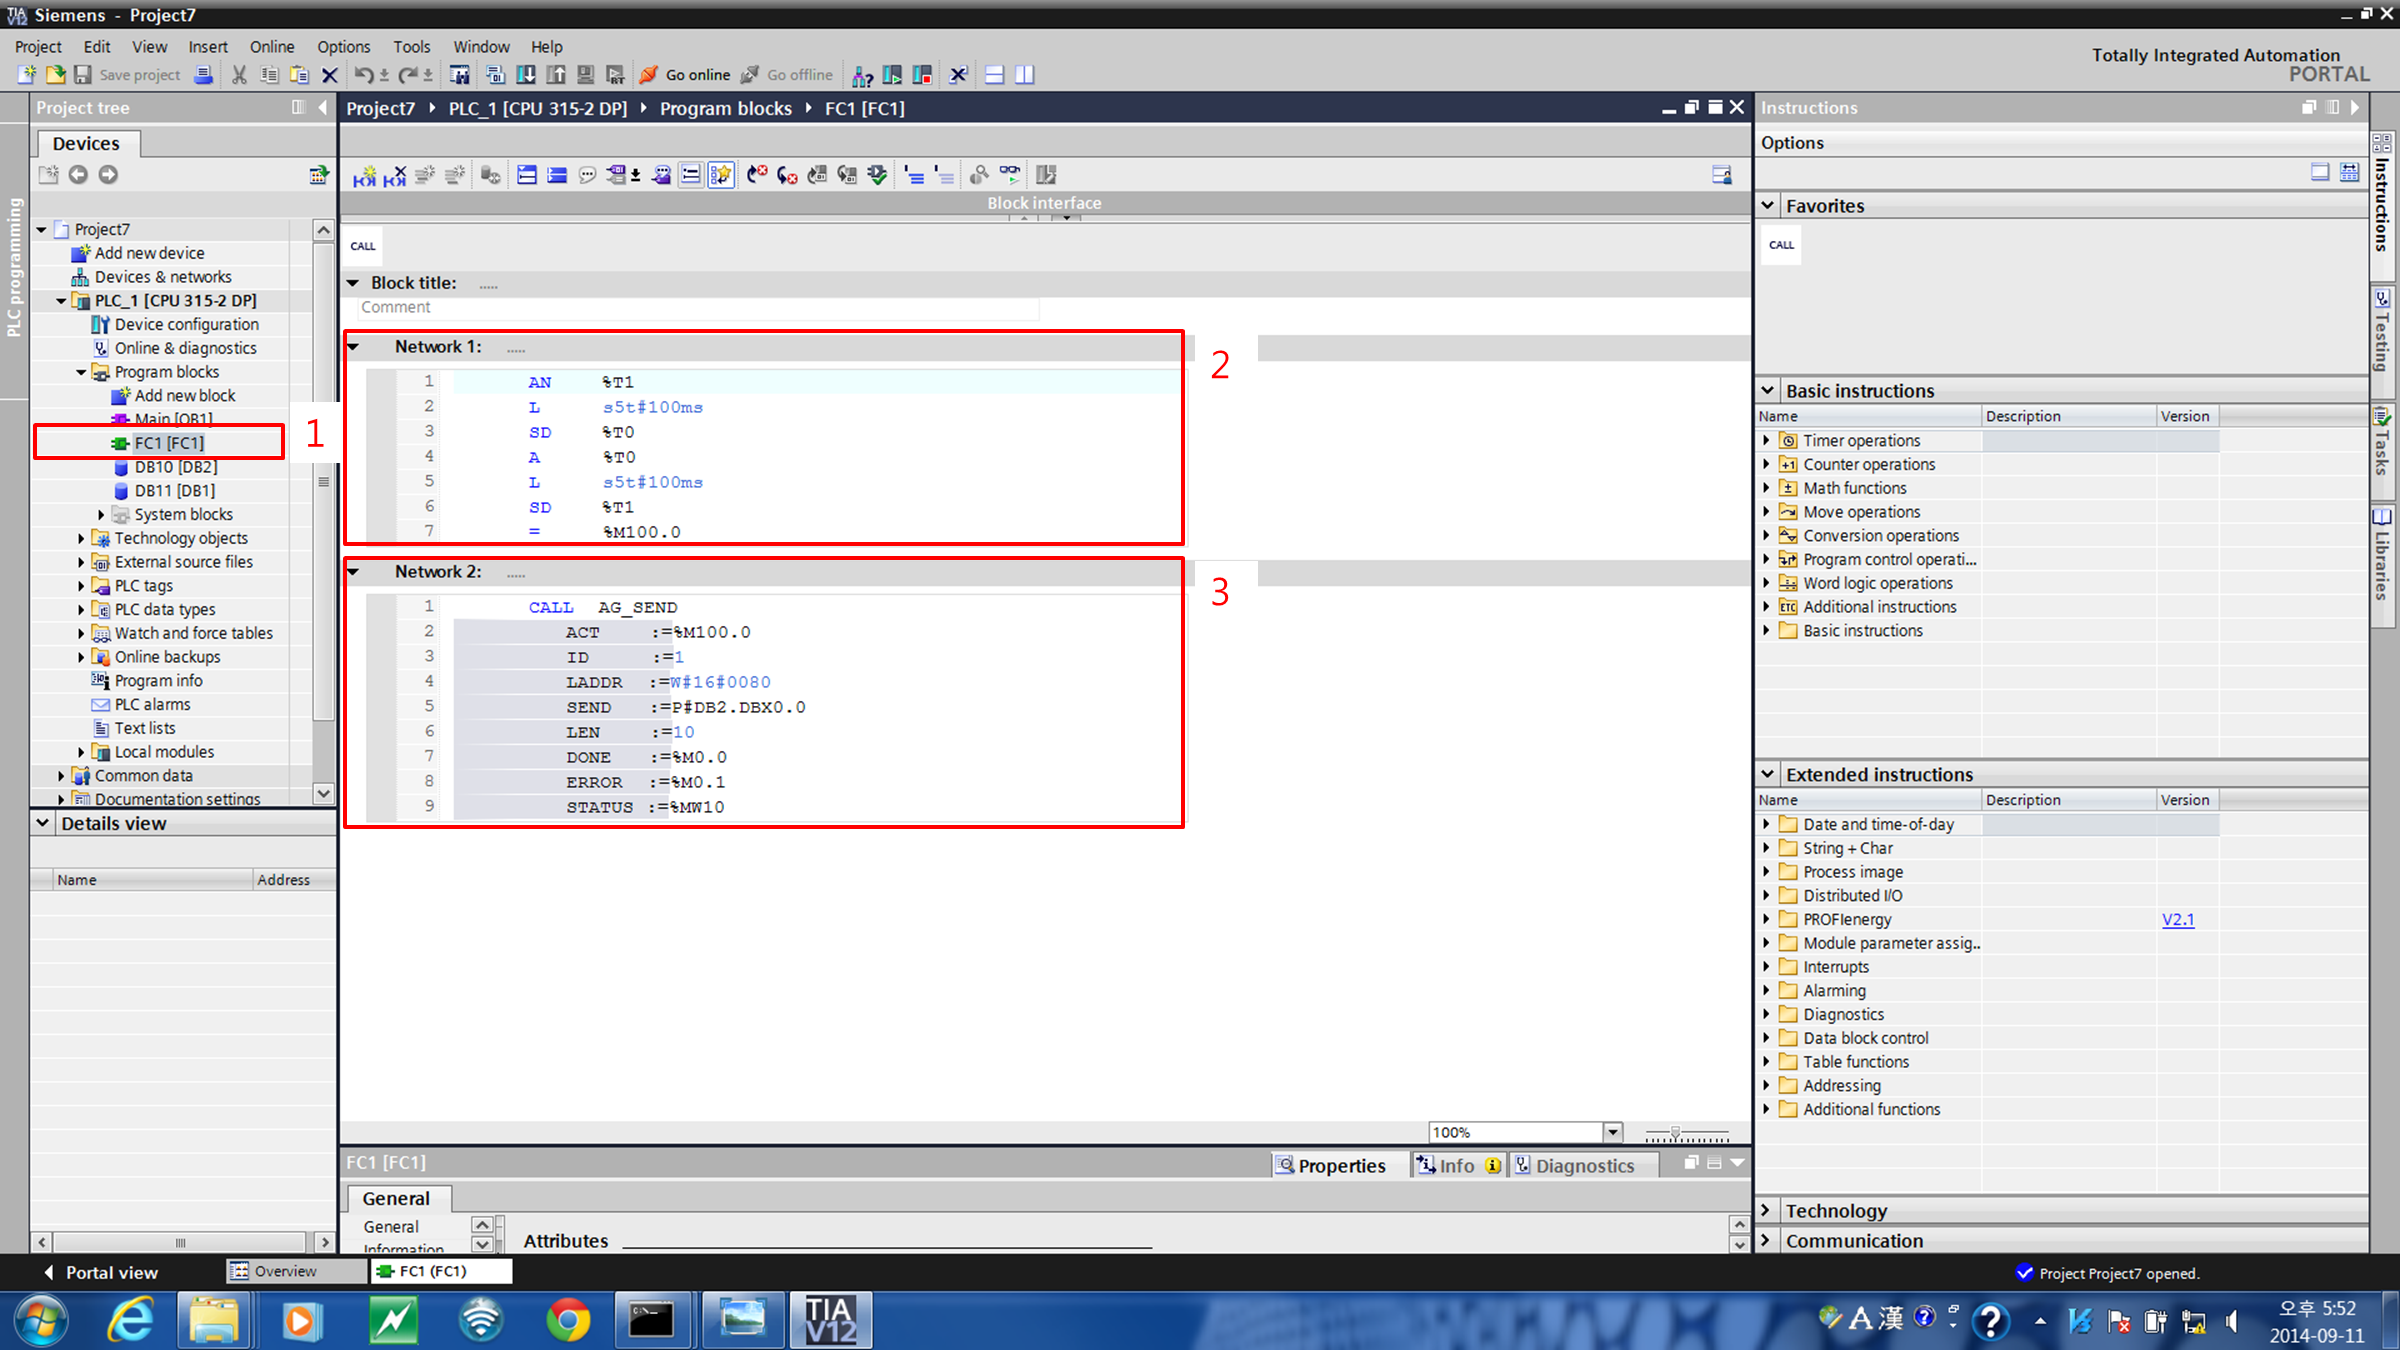
\includegraphics[width=0.96\textwidth]{./images/fig-FC1.png}
  \caption{FC1 program source code}
  \label{}
\end{figure}
\begin{lstlisting}[style=termstyle]
Network1:
	AN	%T1
	L	s5t#100ms
	SD	%T0
	A	%T0
	L	s5t#100ms
	SD	%T1
	=	%M100.0

Network2:
	CALL	AG_SEND
	ACT	:=%M100.0
	ID	:=1
	LADDR	:=w#16#0080
	SEND	:=P#DB2.DBX0.0
	LEN	:=10
	DONE	:=%M0.0
	ERROR	:=%M0.1
	STATUS	:=%MW10
\end{lstlisting}
Step5. \verb|DB10|을 더블클릭하여 Fiure 18 과 같이 Struct를 구성한다. 이 struct는 여러가지 유형의 데이타 타입을 하나의 묶음으로 만든 저장소로 EPICS와의 통신과정에서 필요한 데이터 묶음을 한꺼번에 주고 받는 저장소 역할을 한다.\\
\begin{figure}[!htb]
  \centering
  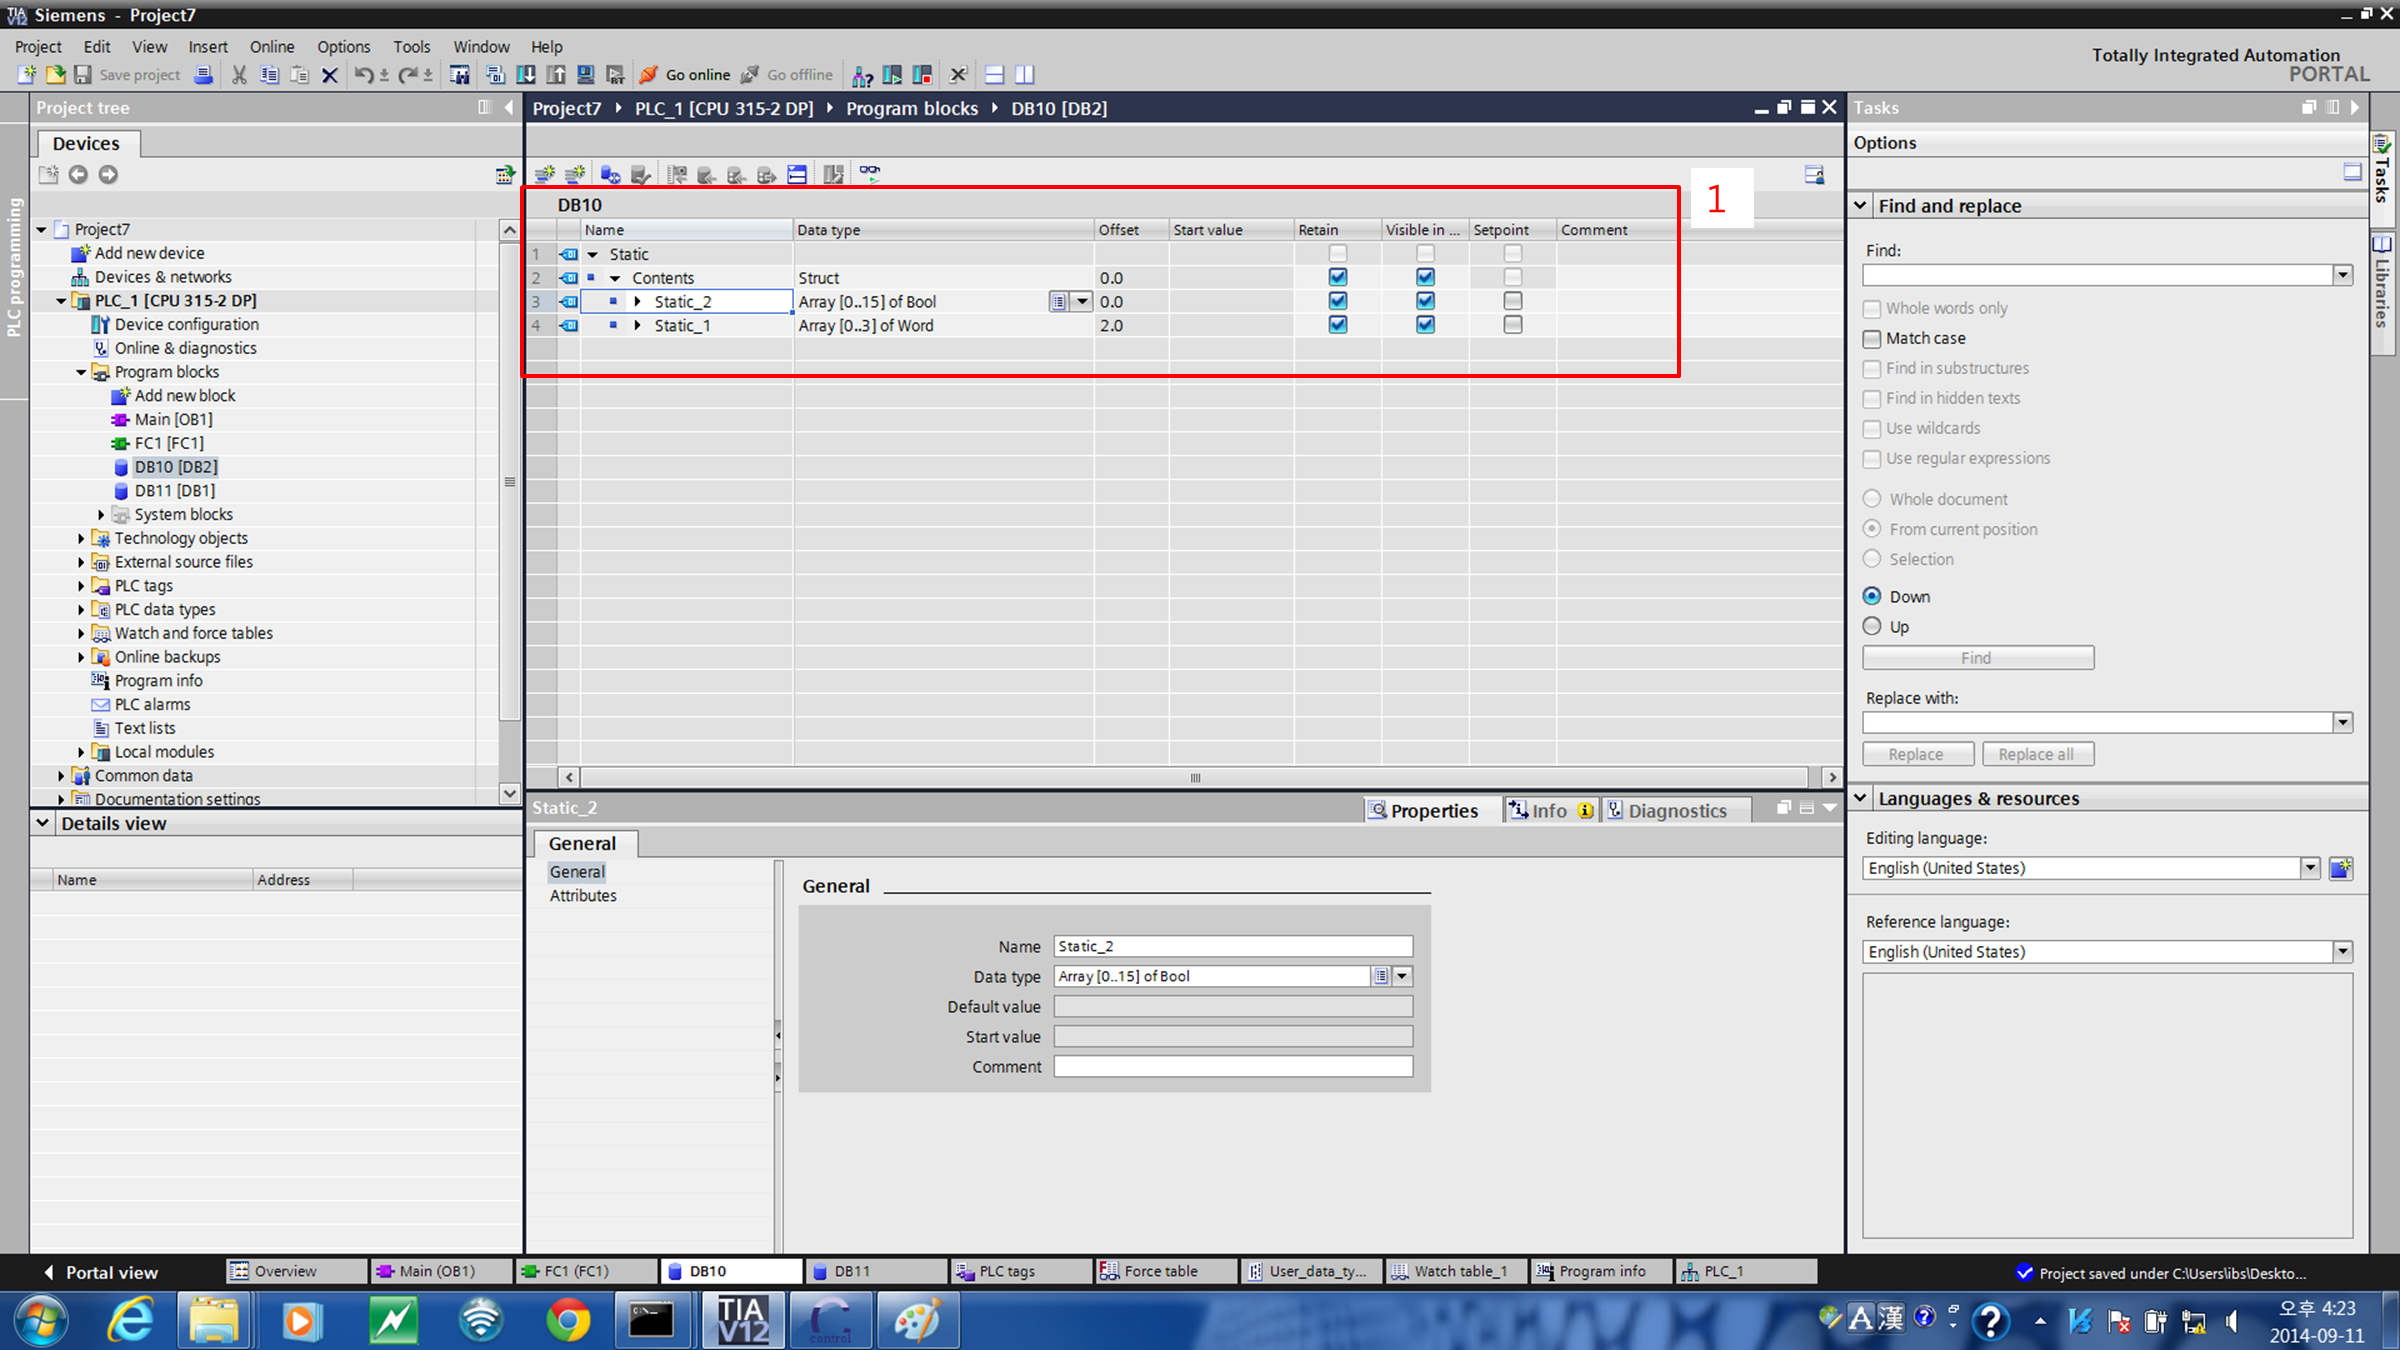
\includegraphics[width=0.96\textwidth]{./images/fig-DB10.png}
  \caption{DB10 data structure}
  \label{}
\end{figure}
\newline Step6. \verb|DB11|을 더블클릭하여 Figure 19 과 같이 struct를 구성한다. Step5의 과정과 동일하다.\\
\begin{figure}[!htb]
  \centering
  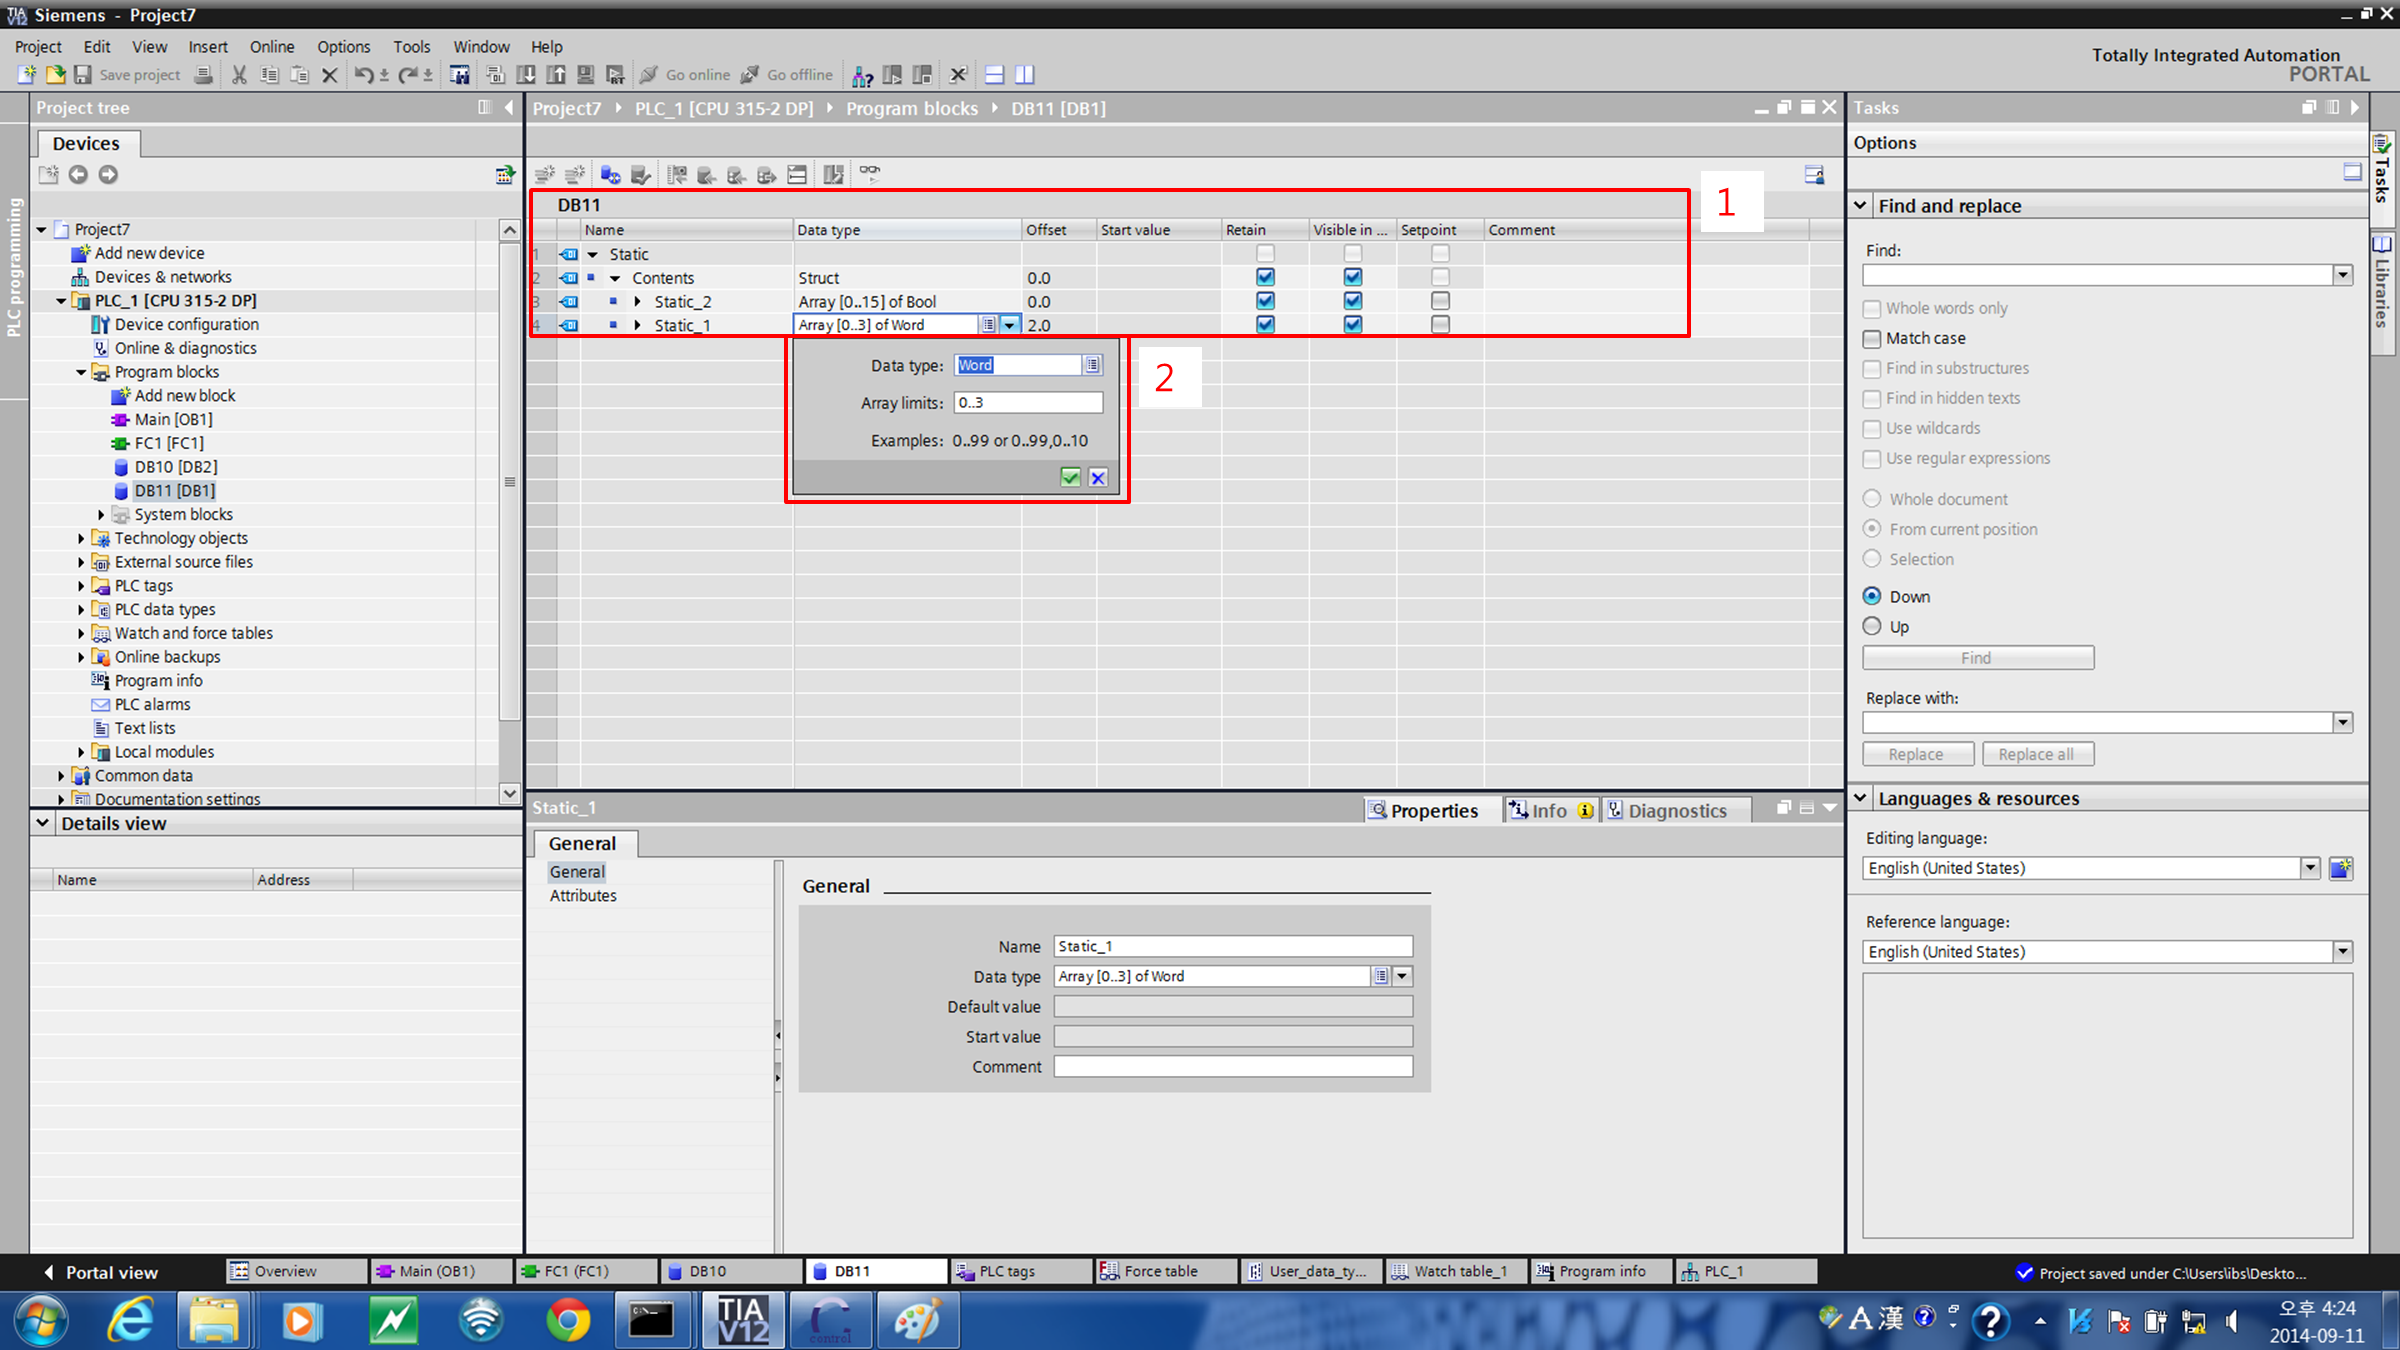
\includegraphics[width=0.96\textwidth]{./images/fig-DB11.png}
  \caption{DB11 data structure}
  \label{}
\end{figure}

\chapter{EPICS 와의 연동}
여기에서는 EPICS와 s7plc의 EPICS드라이버는 설치되어 있는 상태에서 IOC의 설정 내용만을 설명하기로 한다.
EPICS에 관한 정보는 EPICS 홈페이지를 참고하기바라며, s7plc의 EPICS 드라이버에 관한 정보는 PSI 홈페이지를 참고하기 바란다.

\section{st.cmd file 설정}
EPICS IOC 생성후 /iocBoot/ioc/st.cmd 파일에 다음과 같이 설정한다.

\begin{lstlisting}[style=termstyle]
#!../../bin/linux-x86/s7Test

## You may have to change s7Test to something else
## everywhere it appears in this file

< envPaths

cd ${TOP}

dbLoadDatabase "dbd/s7Test.dbd"
s7TestregisterRecordDeviceDriver pdbbase
#s7plcConfigure (PLCname, IPaddr, port, inSize, outSize, bigEndian, recvTimeout, sendIntervall) 
s7plcConfigure "Station1", "10.1.5.203", 2000, 16, 16, 1, 500, 100
dbLoadRecords "db/test1.db"

cd ${TOP}/iocBoot/${IOC}
iocInit
\end{lstlisting}
\begin{itemize}
\item s7plc configuration on st.cmd file
\begin{itemize}
\item inSize        : PLC로부터 읽어오는 byte 크기
\item outSize       : PLC로 쓰는 byte 크기
\item bigEndian     : 1=bigEndian, 0=littleEndian
\item recvTimeout   : PLC로부터 recvTimeout milliseconds이내에 값을 받지 못할 경우 접속을 끊는 시간
\item sendIntervall : 출력을 sendIntervall milliseconds이내에 처리해야하는 시간
\end{itemize}
\end{itemize}

\section{record file 작성}
/db/test1.db 파일을 다음과 같이 작성한다.
 
 
\begin{lstlisting}[style=termstyle]
 ${TOP}/db
\end{lstlisting}

\begin{lstlisting}[style=termstyle]
record(bi, s7-status) {
	        	field(DTYP, "S7plc stat")
		        field(INP, "@Station:0")
			field(SCAN, "I/O Intr")
		        field(ZNAM, "disconnected")
		        field(ONAM, "connected")
		        field(ZSV, "MAJOR")
		        field(FLNK, "s7-status-counter")
}
record(calc, s7-status-counter) {
		        field(INPA, "s7-status-counter")
	  	        field(CALC, "A+1")
		        field(FLNK, "s7-disconnect-counter")
}
record(calc, s7-disconnect-counter) {
		        field(INPA, "s7-status")
		        field(INPB, "s7-disconnect-counter.LA")
		        field(INPC, "s7-disconnect-counter")
		        field(CALC, "(A=0&&B=1)?C+1:C")
}
record(bi, bi-1) {
		        field(SCAN, "I/O Intr")
		        field(DTYP, "S7plc")
		        field(INP, "@Station:0/2 B=0 T=BYTE")
}
record(bi, bi-2) {
		        field(SCAN, "I/O Intr")
		        field(DTYP, "S7plc")
		        field(INP, "@Station:0/2 B=1 T=BYTE")
}
record(bi, bi-3) {
	        	field(SCAN, "I/O Intr")
			field(DTYP, "S7plc")
		        field(INP, "@Station:0/2 B=2 T=BYTE")
}
record(bi, bi-4) {
		        field(SCAN, "I/O Intr")
		        field(DTYP, "S7plc")
		        field(INP, "@Station:0/2 B=3 T=BYTE")
}
record(bo, bo-1) {
		        field(DTYP, "S7plc")
		        field(OUT, "@Station:0/2 B=0 T=BYTE")
		        field(PINI, "YES")
}
record(bo, bo-2) {
		        field(DTYP, "S7plc")
		        field(OUT, "@Station:0/2 B=1 T=BYTE")
			field(PINI, "YES")
}
record(bo, bo-3) {
	        	field(DTYP, "S7plc")
			field(OUT, "@Station:0/2 B=2 T=BYTE")
			field(PINI, "YES")
}
record(bo, bo-4) {
		       field(DTYP, "S7plc")
		       field(OUT, "@Station:0/2 B=3 T=BYTE")
		       field(PINI, "YES")
}

\end{lstlisting}

\end{document}
